\section{Limitations}
\label{sec:app_limitations}
% =============================================================================

The main paper acknowledges three limitations (\cref{sec:conclusion}). Here we expand on each and identify additional caveats that qualify the claims.

\paragraph{Single-domain evidence.}
All experiments use chess as the primary testbed. The framework---subagent with extractable representations, lightweight projector, end-to-end RL---is domain-agnostic in principle, but a complete multi-task evaluation beyond chess remains future work. The framework has not been tested in continuous action spaces (e.g., robotics) or multi-agent adversarial settings beyond two-player zero-sum games. The claim that internalization outperforms verbalization is established for chess; generalization to other domains is a hypothesis, not a finding.

\paragraph{Closed-source agent requirement.}
LLAMIA requires access to the agent's internal activations (the penultimate-layer representation $\vh_s$). This precludes application to closed-source agents that expose only API endpoints.
% \somesh{TODO: Add a paragraph here showing the deployment path: Frontier LLM <-> LLAMIA <-> Lc0, where LLAMIA bridges open-source agents to closed-source frontier models via natural language on one side and latent internalization on the other.}

\paragraph{Scale limitations.}
The largest LLAMIA model is 14B parameters. We do not evaluate whether the verbalization debt persists, shrinks, or grows at larger scales (32B, 70B, 400B). It is plausible that sufficiently large LLMs can partially compensate for verbalization loss through better in-context reasoning, which would qualify the bottleneck claim as scale-dependent rather than absolute. The matched-recipe comparison (LLAMIA vs.\ LLAMIA-Verb at the same scale) controls for this within our range, but extrapolation is uncertain.

% =============================================================================

\section{Ablations}
\label{sec:app_ablations}
% =============================================================================

\subsection{Dynamic Re-Encoding (InvokeAgent)}
\label{sec:app_abl_invoke}

\subsubsection{Static vs.\ Dynamic}
\label{sec:app_abl_invoke_static}

\subsubsection{Invocation Frequency}
\label{sec:app_abl_invoke_freq}

\subsection{Latent vs.\ Symbolic-Rich Matched Information (C3)}
\label{sec:app_abl_symbolic}

\subsection{Projection Token Count}
\label{sec:app_abl_tokens}

\subsection{Agent Size and Playing Strength}
\label{sec:app_abl_agentsize}

\subsection{Sensitivity Sweeps}
\label{sec:app_abl_sweeps}

\subsubsection{Projector Capacity}
\label{sec:app_abl_sweeps_projector}

\subsubsection{Data-Axis Scaling}
\label{sec:app_abl_sweeps_data}

\subsubsection{LoRA vs.\ Full Fine-Tuning}
\label{sec:app_abl_sweeps_lora}

\subsubsection{Decoding Robustness}
\label{sec:app_abl_sweeps_decoding}

% =============================================================================

\section{Human Evaluation Study}
\label{sec:human_study}

We conduct a human evaluation study to validate LLAMIA's commentary generation against automatic metrics. Unlike subjective preference studies, we design task-based evaluations that measure whether commentary enables accurate game understanding.


\subsection{Participants and Protocol}
\label{sec:study_participants}


We recruit 12 participants from two institutions with \url{chess.com} affiliated programs. All participants meet the following criteria: (1) peak online rating of 1600+ on chess.com or lichess.org, (2) over 20,000 online games played, and (3) prior annotation experience on GameKnot.com's game analysis platform. Participants were presented with a study protocol and signed IRB approval from the participating institution, which detailed the data collection procedures and usage terms.


\subsection{Commentary Evaluation Tasks}
\label{sec:commentary_tasks}


We compare commentary from three sources: Human expert commentary (from the Agadmator dataset), LLAMIA-13B, and GPT-4o with Lc0 tool access. For each of 50 game segments (15--25 moves), participants complete three tasks designed to measure functional understanding rather than subjective preference.

\paragraph{Task 1: Position Evaluation from Commentary (Accuracy).}
We test whether commentary accurately conveys positional assessment. At 5 randomly selected positions within each game segment, participants read only the commentary (no board visible) and predict the engine evaluation on a 7-point scale: decisive White advantage ($> +3$), clear White advantage ($+1.5$ to $+3$), slight White advantage ($+0.5$ to $+1.5$), equal ($-0.5$ to $+0.5$), slight Black advantage, clear Black advantage, decisive Black advantage. We measure RMSE between predicted and actual centipawn evaluations (scaled to the 7-point range).

\paragraph{Task 2: Move Prediction from Commentary (Insight).}
We test whether commentary explains strategic rationale well enough to guide move selection. At 5 positions per segment, participants read the commentary describing the current position and are presented with three legal move options (the played move plus two engine-suggested alternatives). Participants predict which move was played based on the commentary's description of plans and threats. We report prediction accuracy.

\paragraph{Task 3: Quality (Engagement).}
Participants rate each commentary segment on a 5-point Likert scale: ``This commentary would help a 1400-rated player understand the strategic themes of this game.'' This captures perceived pedagogical value.


\subsection{Results}
\label{sec:study_results}


\begin{table}[h]
\centering
\begin{adjustbox}{max width=0.98\textwidth}
\begin{tabular}{l|cc|c}
\toprule[1.2pt]
\textbf{Commentary Source} & \textbf{Eval Prediction} & \textbf{Move Prediction} & \textbf{Educational Value} \\
 & (RMSE $\downarrow$) & (Accuracy $\uparrow$) & (Likert 1-5 $\uparrow$) \\
\midrule
Human (Agadmator) & \valbest{0.89} & \valbest{71.2\%} & \valbest{4.31} \\
LLAMIA-13B & \valgood{1.12} & \valgood{64.8\%} & \valgood{3.89} \\
GPT-4o + Lc0 & 1.47 & 58.3\% & 3.42 \\
\midrule
Random Baseline & 2.31 & 33.3\% & -- \\
\bottomrule[1.2pt]
\end{tabular}
\end{adjustbox}
\caption{\textbf{Commentary Evaluation Results.} LLAMIA-13B achieves lower evaluation prediction error (1.12 vs 1.47 RMSE) and higher move prediction accuracy (64.8\% vs 58.3\%) than GPT-4o + Lc0, approaching human expert performance (0.89 RMSE, 71.2\% accuracy). Educational value ratings follow the same pattern (3.89 vs 3.42 Likert). Results are averaged over 12 participants and 50 game segments (250 evaluation points per commentary source). Inter-rater reliability: Krippendorff's $\alpha = 0.74$ for evaluation prediction, $\alpha = 0.81$ for move prediction.}
\label{tab:commentary_study}
\end{table}

\paragraph{Analysis.}
LLAMIA's advantage over GPT-4o + Lc0 is most pronounced on evaluation prediction (24\% lower RMSE), indicating that latent-grounded commentary better conveys positional assessment than tool-calling approaches. The gap narrows on move prediction (6.5\% higher accuracy), suggesting both systems adequately describe immediate tactical considerations. Human commentary remains superior, particularly on evaluation prediction (21\% lower RMSE than LLAMIA), reflecting experts' ability to synthesize complex positional factors into coherent narratives.

\paragraph{Qualitative Patterns.}
Participants noted that LLAMIA commentary more frequently mentions specific positional features (``weak d5 square'', ``backward e-pawn'') compared to GPT-4o + Lc0, which tends toward generic assessments (``White has a slight advantage''). However, human commentary excels at narrative continuity, connecting individual moves to longer-term strategic arcs.
\section{Qualitative Examples}
\label{sec:app_examples}
% =============================================================================

\section{Prompts and Templates}
\label{sec:app_prompts}
% =============================================================================

Three prompt regimes govern the pipeline: Stage~1 projector alignment, Stage~2 GRPO
rollouts, and the shared dynamic re-encoding (InvokeAgent) format.

%------------------------------------------------------------------------------
\subsection{Stage 1: Projector Alignment}
\label{sec:app_prompts_stage1}

Stage~1 trains the LatentBridge projector ($H_\varphi$, the linear adapter mapping BT4
residual activations into the LLM token space) via supervised learning on chess
instruction data.
Each episode presents several independent questions about the same board position; the
\texttt{<state>} placeholder marks the $k{=}32$ latent tokens projected from the BT4
residual stream and inserted into the LLM's context at that point.
Four question types are sampled per FEN: position evaluation, principal variation, legal
moves, and brief verbal description.
Move notation alternates UCI and SAN with probability 70\,/\,30\,\%; evaluations are in
pawn units.

\begin{tcolorbox}[promptbox,
  title={$\triangleright$\; Stage 1 System Prompt --- Projector Alignment}]
\begin{quote}
You are LLAMIA, a chess reasoning assistant.
The board state is encoded in the \texttt{<state>} token sequence embedded in the
user's message.
Answer the question about this position precisely and concisely.
Do not narrate your reasoning; give the answer directly.
\end{quote}
\end{tcolorbox}

\begin{tcolorbox}[notebox, title={Stage 1 Training Format (single episode over one FEN)}]
\small
\textbf{User:}~What is the evaluation of the following position?
Describe the evaluation followed by the continuation in UCI format, e.g.\
\emph{``Evaluation is +1.5, Advantage for White, e2e4 e7e5''}. \texttt{<state>}\\[3pt]
\textbf{LLAMIA:}~Evaluation is $+0.5$, white has a slight advantage,
\texttt{d5c6 b4c4 e4d6 c4d3 \ldots}

\tcbline
\textbf{User:}~Give me the principal variation(s); just the evaluation(s) and the
line(s). \texttt{<state>}\\[3pt]
\textbf{LLAMIA:}~$+0.4$, \texttt{e4d6 a3a4 d5c6 b4c3 c6d5 c3d3}

\tcbline
\textbf{User:}~What are the legal moves in this position?
Give me up to 10 comma-separated UCI moves and nothing else. \texttt{<state>}\\[3pt]
\textbf{LLAMIA:}~\texttt{e4f2, d5e6, e4c3, e4g3, e4d6, e4g5, e4d2, e4f6, d5d6, e4c5}

\tcbline
\textbf{User:}~Describe the current position briefly. \texttt{<state>}\\[3pt]
\textbf{LLAMIA:}~It is black's turn. White's King is somewhat exposed, with threats from
Black's Knight and Pawn. Black has a centralised active Knight and Pawn. This position
appears as a complex endgame with White holding a slight advantage due to the extra pawn.
\end{tcolorbox}

%------------------------------------------------------------------------------
\subsection{Stage 2: GRPO System Prompt}
\label{sec:app_prompts_stage2}

\paragraph{Toy task (puzzle popularity / Elo).}
The system prompt below is used verbatim during GRPO rollouts for the toy task
(\S\ref{sec:app_toytask}).
The explicit refusal-suppression clause is required: without it, Qwen3-4B defaults to
``I cannot directly determine\ldots'' and never emits a tool call, collapsing the
format-pass rate to 0\,\% (verified on 20 held-out puzzles at greedy decoding).

\begin{tcolorbox}[promptbox,
  title={$\triangleright$\; Stage 2 System Prompt --- Puzzle Popularity / Elo (GRPO Rollouts)}]
\begin{quote}
You are a chess expert with access to lc0, a top neural network engine.
A puzzle position has been loaded from the FEN in the user's message.
Use the tools below to analyse the position, then estimate the puzzle's popularity and
difficulty rating.

\smallskip
\textbf{Available tools:}
\begin{itemize}[noitemsep,topsep=1pt,leftmargin=14pt]
  \item \texttt{get\_position} --- FEN, ASCII board, legal moves.
  \item \texttt{analyze(nodes, multipv)} --- lc0 MCTS search.
  \item \texttt{get\_policy(nodes)} --- raw NN priors and per-move values.
\end{itemize}

\smallskip
\textbf{You must always provide a numeric answer.}
Refusing or writing ``I cannot determine'' is not permitted ---
give your best guess even if uncertain.

\smallskip
End your reply with exactly one line in the form:\\[2pt]
\texttt{The popularity is \textit{<int>} and the ELO is \textit{<int>}}
\end{quote}
\end{tcolorbox}

\paragraph{Full LLAMIA-Bench.}
All six task families (behaviour cloning, stylometry, puzzle understanding, move
annotation, game commentary, instruction-conditioned planning) share the same tool
catalogue as the toy task.
Task-specific instructions replace the popularity/Elo mandate; the
refusal-suppression clause is retained across all variants.
Full per-task system prompts are \tbd{} pending experimental finalization.

%------------------------------------------------------------------------------
\subsection{InvokeAgent Trigger Format}
\label{sec:app_prompts_invoke}

Dynamic re-encoding (\textsc{InvokeAgent}) fires after every board-mutating tool call
(\texttt{make\_move}, \texttt{undo\_move}, \texttt{reset\_position}).
The harness re-runs the BT4 forward pass on the updated FEN, encodes a fresh set of
$k{=}32$ latent tokens, and prepends them as a \texttt{<state>} prefix to the next user
turn.
Because mutating calls are dispatched sequentially (\S\ref{sec:app_toolcall}), the
re-encoding always sees a fully settled board state.
Read-only calls (\texttt{analyze}, \texttt{get\_policy}, \texttt{get\_position}) do not
trigger re-encoding; the token budget is therefore capped at $k$ additional tokens per
state transition, regardless of analysis depth.

\begin{tcolorbox}[notebox, title={InvokeAgent Turn Structure (blunder-analysis episode)}]
\small
\textbf{Round~1 --- User:} \texttt{<state$_0$>} Why is \texttt{Nxd4} a blunder here?
[FEN $s_0$]\\[3pt]
\textbf{Round~1 --- LLAMIA:} \textit{(emits two parallel \texttt{analyze} calls ---
see \S\ref{sec:app_toolcall_example})}

\tcbline
\textbf{Round~2 --- Tool:} \textit{(harness returns engine evaluations; state unchanged)}\\[3pt]
\textbf{Round~2 --- LLAMIA:} Final answer citing \texttt{Qa5+} / \texttt{Qxg5}.
\end{tcolorbox}

Since no board mutation occurs in blunder analysis, \textsc{InvokeAgent} does not fire.
The re-encoding path is active in multi-step planning episodes, where the agent sequences
\texttt{make\_move} calls to explore a variation before deciding on a recommendation.

\begin{tcolorbox}[notebox, title={InvokeAgent Turn Structure (multi-step planning episode)}]
\small
\textbf{Round~1 --- User:} \texttt{<state$_0$>} Find the best three-move combination.
[FEN $s_0$]\\[3pt]
\textbf{Round~1 --- LLAMIA:} \texttt{make\_move(e2e4)}

\tcbline
\textbf{Round~2 --- Tool:} \{move\_played: \texttt{e4}, fen: $s_1$, \ldots\}\\
\textit{(harness re-encodes $s_1$ $\!\to\!$ fresh \texttt{<state$_1$>})}\\[3pt]
\textbf{Round~2 --- User (injected):} \texttt{<state$_1$>}\\[3pt]
\textbf{Round~2 --- LLAMIA:} \texttt{analyze(multipv=3)}

\tcbline
\textbf{Round~3 --- Tool:} \textit{(engine lines from $s_1$)}\\[3pt]
\textbf{Round~3 --- LLAMIA:} \texttt{undo\_move()}

\tcbline
\textbf{Round~4 --- Tool:} \{fen: $s_0$, \ldots\}\\
\textit{(harness re-encodes $s_0$ $\!\to\!$ fresh \texttt{<state$_0'$>})}\\[3pt]
\textbf{Round~4 --- User (injected):} \texttt{<state$_0'$>}\\[3pt]
\textbf{Round~4 --- LLAMIA:} Final recommendation.
\end{tcolorbox}

\noindent The injected \texttt{<state>} prefix in Rounds~2 and~4 is invisible to the
human user; the harness inserts it programmatically before forwarding the tool result to
the next LLM call, keeping the re-encoding fully transparent to the model's reasoning loop.

% =============================================================================


\section{Dataset}
\label{app:data_stats}
\vspace{-2mm}
In this section, we describe the datasets and on which we train LLAMIA. Extensive research from Flan, LLaVA, QLora \cite{longpre2023flan,dettmers2024qlora,liu2024improved,liu2023visual} demonstrate that joint training across diverse tasks, modalities, and instructions enhances model generalization and zero-shot reasoning. Motivated by this, we train LLAMIA on interleaved datasets that combine agent states, actions, and language instructions. Our approach integrates three objectives: (1) aligning pretrained agents with LLM representations, (2) cloning diverse decision making behaviors, and (3) predicting human explanations. Below we outline the datasets used.

\subsection{Agent-Projector Pretraining}
The pretraining phase aligns the agent’s latent state representations with the LLM’s embedding space. We extract the \textbf{top moves} and their \textbf{pawn evaluations} from the lichess evaluation database \footnote{\url{https://database.lichess.org/\#evals}}. We filter out weaker evaluations to obtain 50 million evaluations. Further, we augment these with positional features such as legal moves, tactical motifs (e.g., pins, forks), and strategic annotations (e.g., king safety, pawn structure) extracted from Chevy\footnote{\url{https://github.com/int8/chevy}}. Listing \ref{listing:pretraining_instruction_format} shows the exact conversation format.

\subsection{Language-Action Fine-Tuning}
\label{subsec:language_action }
\subsubsection{Behavior Cloning}
Behavior cloning is the process of learning policies by mimicking demonstrations. In chess it is used to replicate human-like playstyles, engine strategies, and grandmaster tactics making gameplay more relatable, instructive, and diverse. This dataset is crucial for training LLAMIA to adapt its internal agent’s policy across varying expertise level.

We curate chess games from diverse sources, spanning human and engine play across skill levels. The Lichess dataset includes 12 million rapid and blitz games with Elo ratings between 1000 and 2500. For superhuman play, we incorporate 3 million CCRL games sourced from \cite{feng2024chessgpt},  played by engines like Stockfish and Leela Zero, which have Elo ratings between 2800 and 3700. Additionally, we include 158,000 elite grandmaster tournament games \cite{gmchessgames2022}, providing insights into expert human strategy. Where available, metadata such as player Elo, time control, and annotations are included. Listing \ref{listing:lichess_instruction_format} shows the exact conversation formats. 
During testing, we evaluate behavior cloning on the MAIA-KDD test set \cite{mcilroy2020aligning}.

\subsubsection{Commentary Prediction}
\label{sec:commentary}
While chess engines surpass human play, they lack the ability to provide meaningful, human-like commentary or rationales. Most engines offer numerical evaluations (e.g., `+0.39') but fail to contextualize these values in strategic or positional terms. In contrast, expert commentators interpret engine outputs to articulate insights such as, ``Your isolated pawns outweigh the advantage of a bishop pair and safer king'' transforming raw evaluations into actionable knowledge. Commentary not only enhances understanding but also democratizes learning, making high-level insights accessible to a broader audience. To train LLAMIA in explanatory reasoning over decisions we collect:

\paragraph{State Commentary}: We include 90k annotated games, primarily sourced from Lichess, filtered to include only English annotations \cite{jhamtani-etal-2018-learning}. These annotations provide insights into
various aspects of the game, including move explanations,
game summaries, alternative lines, thematic insights, in-
structional content, and evaluative comments (Listing~\ref{listing:state_annotation_format}).

\paragraph{Game Commentary:} We introduce the first large-scale dataset for game-level commentary with time- and move-stamped explanations, comprised of 2000 narrated games from Agadmator’s YouTube channel. We extract paired commentary from the transcripts by aligning video clips with natural language transcripts based on timestamps. Listing \ref{listing:commentary_format}. Since move segmented commentary is not available we detail our algorithm for creating this, we maintain a move by move buffer over segments of moves to track the commentated game so far. Then for each segment of the game we ask GPT-4o to annotate the moves that are in the PGN of the game as well as transcript (extracted using whisper-v3-large) in square brackets. Next we match the moves in PGN and eliminate retry where the move order is not same as PGN and annotated commentary. 

\subsubsection{Puzzle Understanding}
Chess puzzles have long been used to assess understanding in both humans and engines. These puzzles consist of specific board positions with an objectively winning sequence of moves (typically only one solution) and are characterized by themes, difficulty, and interestingness.

We curate a dataset of 4 million puzzles from Lichess \footnote{\url{https://database.lichess.org/lichess_db_puzzle.csv.zst}}, each sourced from real gameplay and enriched with metadata such as popularity, opening tags (for puzzles within the first 20 moves), and difficulty ratings. The interestingness score, ranging from -100 (worst) to 100 (best), is computed from upvotes and downvotes, weighted by solver performance. Puzzle difficulty is determined using a Glicko-2 rating system, where each solving attempt is treated as a rated match between the solver and the puzzle. 

\subsection{Language and Conversational Data}
Recent work by \citet{feng2024chessgpt} attempts bridging language and policy by fine-tuning solely on language data. Additionally, training on diverse web-scale content has improved generalization in prior foundation models \cite{liu2024improved}. Since curating high-quality action fine-tuning datasets is challenging, we also incorporate diverse chess-related language-only datasets from the web, including

\textbf{Chess Stack Exchange}: Expert discussions and Q\&A threads sourced from \cite{feng2024chessgpt}.We use 9k StackExchange questions.

\textbf{Web}: Extracted chess-related content from the RedPajama-v2 dataset \cite{weber2024redpajama} .To extract chess-related language corpus, we filter using the header for the keyword ’chess’.

\textbf{Transcripts}: 100 hours of chess commentary from Chess24 and chess.com streams. \cite{feng2024chessgpt} also uses books, chessable forums, and transcripts that are not publicly available. To ensure fair experimental comparisons, we exclude these.

\textbf{Chat Dataset}:
To preserve the multi-turn conversational structure and general textual reasoning capabilities, we augment our fine-tuning dataset with 70k ShareGPT conversations, aligning with the dataset used in the base chat model Vicuna \cite{zheng2023judging}.


% \begin{enumerate}
%     \item Results and Discussion: Baselines and Ablations are not clear \somesh{Summary Table?}, due to which people did not understand ChessGPT and other baselines. SFT without TC, SFT with TC, Verbalization \somesh{Results added in individual tables}
%     \item Add baseline for SFT + Tool-Calling \somesh{Added}
%     \item Results and Discussion: Table in main paper\somesh{Summary Table?}, Figure 6 Janus label is wrong and unreferenced \somesh{XXX}
%     \item Behavior Cloning table: Peaking Behavior, Explain the buckets from \cite{jacob2022modeling}. \somesh{Updated Buckets will remove 2250/2500 and rename}
%     \item Related work: Unified-IO2 comments, \somesh{XXX} 
%     \item How representative is the example in Fig. 4, @Harini: Put the cherry picking rationale \somesh{XXX}
%     \item Explain table 7 in detail, add paragraph in results and discussion \somesh{XXX}
%     \item Improve the qualitative example. \somesh{XXX}
%     \item Data Appendix \somesh{XXX}
%     \item Explain LLAMIA Bench \somesh{XXX}
%     \item Introduction: Lora adapters / Task expertise + Results \somesh{XXX Will strip off main text in case of reviews, was a one off concern}
%     \item Input vs Output vs State in Architecture \somesh{XXX}
%     \item Extending to other envs \somesh{XXX}
%     \item Output Projections as a part, as thinking chains \somesh{XXX}
%     \item Stylometry: Explain why some of the results are not good \somesh{Removed}
%     \item Metrics explanation for Commentary \somesh{Will update to G-eval + Highlights}
%     \item Instruct Conditioned Planning: When is the engine swapped \somesh{XXX Eval sections}
%     \item Qualitiative and Quant results on Image aesthetics and Behavior \somesh{XXX Adding figures}
% \end{enumerate}


\section{Tables, Figures and Evaluation Setup}
Here we describe the quantitative results, baselines and evaluation setups comprehensively.
\subsection{Baselines} First we detail the baselines we use for the experiments.
\paragraph{ICL: Few Shot LLM} We follow the standard LLM few shot technique. For each task we calibrate the number of shots using 50 examples on a held out test set.
\paragraph{ICL + Tool Calling: Few Shot LLM + Tool Calling}
Here we use ReACT \cite{wu2023autogen} and Autogen \cite{wu2023autogen} to implement tool calling and ICL.
\paragraph{IFT: ChessGPT}
Here we use \cite{feng2024chessgpt} for the 3B models to test the improvement compared to only IFT with text tokens as described in \cref{eq:llm_agent_objective}. However, the complete dataset was not made public, and they only provide checkpoints for 2b and 3b model, so for a fair comparison we finetune 7B and 13B models with our dataset. To replace the agent, we add the FEN, the complete verbalization as shown in \cref{listing:pretraining_instruction_format}, and next best moves and evaluations alongside while finetuning and doing inference.
\paragraph{LoRA: LLAMIA LoRA models} We use LoRA with Rank 32 for our experiments.


\label{sec:addl-results}
\FloatBarrier
\subsection{Gameplay}
\label{app:gameplay_eval}
We use the following metrics to evaluate our models and/or measure pretraining (stage-1) progress on their competitive gameplay.

\paragraph{Action ranking (Kendall's $\tau$)}
The average test set rank correlation of the predicted action distribution with the ground truth given by our agent Lc0-BT4. Kendall's $\tau$ ranges from -1 (exact inverse order) to 1 (exact same order), with 0 indicating no rank correlation. The ground-truth ranking is given by evaluating $\pi^\text{G}(s,a)$ for all legal actions. The predicted ranking is obtained by evaluating the probability for all valid actions $F(a|s, \text{prompt})$ through greedy decoding.

\paragraph{Puzzle accuracy}
We evaluate LLAMIA on its capability to solve puzzles from a collection of Lichess puzzles that are rated by Elo difficulty from $399$ to $2867$ based on how often each puzzle has been solved correctly. We use \emph{puzzle accuracy} as the percentage of puzzles where the action sequence exactly matches the \emph{entire} solution action sequence. We use $1$K puzzles for our results. Compared to \cite{ruoss2024grandmaster}, we have 0\% overlap in the train and test distributions of puzzles.

\paragraph{Game playing strength (Elo)}
We evaluate the playing strength (measured as an Elo rating) of the policies by running an internal tournament between all the agents from \cref{tab:gameplay-performance}, except for GPT-4o. The majority of the results are obtained from \cite{ruoss2024grandmaster}; we only evaluate LLAMIA against each of the agents, with $1000$ games per pair, and compute the Elo with BayesElo~\citep{coulom2008whole} using the default confidence parameter of $0.5$. To ensure variability in the games, we use the openings from the Encyclopaedia of Chess Openings~(ECO)~\citep{matanovic1978eco}.


\begin{table*}[!h]
    \centering
    \begin{adjustbox}{max width=1.05\textwidth}
    \begin{tabular}{lcccrrcc}
    \toprule[1.2pt]
    \textbf{Agent} & \textbf{Train} & \textbf{Search} & \textbf{\#FEN} & \textbf{\#Params} & \textbf{Tournament Elo} & \textbf{Puzzle(\%)} \\
    \midrule
    LLAMIA-7B [Ours] & SALT & & 30M & 7B & 2171~($\pm31$) & 90.1 \\
    LLAMIA-13B [Ours] & SALT(LoRA) & & 30M & 8M & 2058~($\pm41$) & 88.9 \\
    LLAMIA-13B [Ours] & SALT & & 30M & 13B & \valgood{2279~($\pm45$)} & 92.9 \\
    \midrule[1pt]
    Transformer-9M  & SL & & 15B & 9M & 2025~($\pm18$) & 88.9 \\
    Transformer-136M & SL & & 15B & 136M & 2259~($\pm16$) & \valgood{94.5} \\
    Transformer-270M & SL & & 15B & 270M & \valbest{2299~($\pm15$)} & \valbest{95.4} \\
    \midrule
    GPT-4o & ICL & & - & - & 1310$(\pm92)$ & 51.9 \\
    AlphaZero (policy only) & RL & & ~300M & 65M & 1777~($\pm25$) & 56.1 \\
    AlphaZero (value only) & RL & & ~300M & 65M & 1992~($\pm19$) & 82.0 \\
    AlphaZero ($400$ MCTS) & RL & \checkmark & ~300M & 65M & 2470~($\pm16$) & 95.6 \\
    \midrule
    Lc0 T82 (policy only) & RL & & 2.87B & 109M & 2292~($\pm16$) & 88.6 \\
    Lc0 T82 (value only) & RL & & 2.87B & 109M & 2418~($\pm16$) & 95.9 \\
    Lc0 T82 ($400$ MCTS) & RL & \checkmark & 2.87B & 109M & 2858~($\pm20$) & 99.6 \\
    \midrule
    SF-16 ($50$ms per move) & SL & \checkmark & 20B & 10.5M & 2711~($\pm18$) & 99.8 \\
    SF-16 ($1.5$s per move) & SL & \checkmark & 20B & 10.5M & 2935~($\pm23$) & 100.0 \\
    \bottomrule[1.2pt]
    \end{tabular}
    \end{adjustbox}
    \caption{\textbf{Gameplay:} We evaluate LLAMIA's performance in competitive chess by comparing its gameplay strength and puzzle-solving. LLAMIA fares better or matches the performance of well established agents like Lc0/AlphaZero and the recent transformer based models \cite{ruoss2024grandmaster} despite training on \underline{100-500x} lesser positions demonstrating stronger generalization and data efficiency. We follow \citet{ruoss2024grandmaster}'s evaluation protocol for tournament Elos.}
    % \yaman{1 liner about the task. Remove Lichess Elo column - if needed, add as another table in appendix - not here. Use colors to denote better, best. Training params should come next to \#training FEN, } LLAMIA shows much stronger or comparable strength generalization matches the gameplay strength of larger Transformers and RL agents while using no search and training on just 30M positions—over 50x fewer than other agents—demonstrating stronger generalization and data efficiency. Comparison of LLAMIA against SF-16 (Stockfish 16), Lc0 (Leela Chess Zero), AlphaZero, (\cite{ruoss2024grandmaster}Deepmind) Chess Transformers, and GPT-3.5-turbo-instruct (following \cite{carlini2023chess}). 270M Transformer exhibits a 2895 Blitz Elo against humans. Lichess (blitz) Elo ratings result from playing against either human opponents or bots on Lichess. Tournament Elo ratings are obtained by making the agents (except GPT3.5 and Deepmind) play against each other and cannot be directly compared but are proportional to the Lichess Elo. Unlike previous engines LLAMIA and Chess Transformers use no test time optimization or search. Further LLAMIA shows a comparable performance in less than 0.2\% of training FENs compared to the latter, this indicates a much higher scope of generalization as opposed to memorization.}
    \label{tab:gameplay-performance}
\end{table*}

\subsection{Game Level Commentary}
From our game commentary dataset described in \cref{sec:commentary}, we extract 100 unpopular games (sorted by views) to avoid overlap with LLM pretraining datasets. We split the entire commentary into segments with a maximum of 25 moves and 2048 tokens, enabling faithful evaluation from GPT-4o. We then evaluate the ground truth and generated commentary using the following metrics:

\paragraph{G-eval}
Our evaluation approach mirrors GCC-Eval \cite{kim2024bridging} to ensure accurate chess commentary evaluation, focusing on informativeness and linguistic quality. However, we do not use Chess.com commentaries, as we already have expert-level commentaries extracted from Agadmator's channel\footnote{\url{https://www.youtube.com/@agadmator}}. The evaluation covers four dimensions: relevance, completeness, clarity, and fluency. While clarity and fluency are general linguistic measures, relevance and completeness require an understanding of chess. We employ GPT-4o with Lc0-BT4 tool calling alongside the ground truth commentary.

\paragraph{Quality}
To measure how accurately the generated commentary explains the state or the value of a position to a novice listener, we first note that GPT-4o demonstrates amateur-level understanding in \cref{tab:gameplay-performance}. Given a commentary segment, we ask GPT-4o to predict the centipawn evaluation and measure the RMSE between the predicted and actual evaluations of the board position at that point. We follow the prompting setup given in \cref{listing:pretraining_instruction_format}, with the commentary appended as described in \cref{tab:game_commentary_annotation}.

\paragraph{Highlight}
To assess how well the commentary addresses audience interest, we prompt GPT-4o to predict audience engagement on a scale from 0 to 100. We extract the ground truth engagement from YouTube using replay graphs and evaluate the RMSE, following the same setup as \citet{singh2024teaching}.

\paragraph{BLEU-2}
We follow the standard NLG BLEU-2 evaluation between each commentary segment.

\begin{table*}[!h]
    \centering
    \begin{adjustbox}{max width=0.98\textwidth}
    \begin{tabular}{lcc|cccc}
    \toprule[1.2pt]
    \textbf{Model} & \textbf{\#Param} & \textbf{Method} & \textbf{G-eval $\uparrow$} & \makecell{\textbf{Quality}\\(RMSE) $\downarrow$} & \makecell{\textbf{Highlight}\\(RMSE) $\downarrow$} & \textbf{BLEU-2 $\uparrow$} \\
    \midrule
    ChessGPT-7B & 7B & IFT & 0.37 & 8.17 & 21.97 & 31.03 \\
    ChessGPT-13B & 13B & IFT & 0.42 & 7.11 & 19.10 & 35.90 \\
    ChessGPT-7B + Lc0 & 7B & IFT + Tool & 0.43 & 7.85 & 20.10 & 33.50 \\
    \midrule
    GPT-4o & - & 1-shot ICL & 0.41 & 4.13 & 19.30 & 20.75 \\
    GPT-4o + Lc0 & - & 1-shot + Tool & \valgood{0.52} & - & 12.31 & 21.03 \\
    LLaMA-3.1 & 405B & 1-shot ICL & 0.41 & 3.99 & 17.10 & 23.90 \\
    LLaMA-3.1 + Lc0 & 405B & 1-shot + Tool & 0.44 & - & 14.47 & 25.07 \\
    \midrule
    LLAMIA-7B & 7B & SALT & 0.49 & \valgood{1.83} & \valgood{8.13} & \valgood{44.93} \\
    LLAMIA-13B & 13B & SALT & \valbest{0.61} & \valbest{0.91} & \valbest{5.09} & \valbest{57.03} \\
    \bottomrule[1.2pt]
    \end{tabular}
    \end{adjustbox}
    \caption{
    \textbf{LLAMIA-Bench game level commentary evaluation}  
    We introduce a new benchmark task for game-level commentary generation, which includes over \(\sim\)500 hours of annotated chess gameplay. This task evaluates not only the coherence and fluency (BLEU-2, G-eval\cite{liu2023g}) but also its measure of correctness and audience impact. We employ G-eval similar to \cite{kim2024bridging}
    \textbf{Quality (Eval RMSE)} assesses how accurately the commentary communicates the game’s progression to a novice listener—estimated by prompting GPT-4o to infer final game evaluation given the commentary segment.  
    \textbf{Highlight (Replay RMSE)} reflects human interest by predicting YouTube replay graph averages from the commentary (0–100 scale) and computing RMSE versus ground-truth.  
    LLAMIA-13B significantly outperforms all baselines, achieving 0.61 G-eval and 57.03 BLEU, while reducing highlight RMSE to 5.09 suggesting it generates not only fluent but strategically informative and attention-worthy narratives. 
    }
    \label{tab:game_commentary_annotation}
\end{table*}

\subsection{Behavior Cloning}
We evaluate behavior cloning on the MAIA-KDD test set \cite{mcilroy2020aligning}. To test the generalization capabilities of models in behavior cloning, we construct the LLAMIA-Bench Behavior Cloning benchmark, which includes three well-known and popular policies or behaviors that are limited in the abundance of available samples. We follow the MAIA evaluation setup of move-matching accuracy for both the test set and the LLAMIA-Bench splits.

\paragraph{GM-25}
The top 25 rated grandmasters in the history of chess\footnote{\url{https://en.wikipedia.org/wiki/List_of_chess_players_by_peak_FIDE_rating}}. We evaluate the capability of LLMs to clone the playing styles of individual grandmasters such as Magnus Carlsen and Viswanathan Anand. The highest number of games played (4641) by an individual is by Viktor Korchnoi\footnote{\url{https://www.365chess.com/top-chess-players-games.php}}, which is less than 3% of the training data required for current state-of-the-art models \cite{mcilroy2020aligning}.

\paragraph{Low-Time}
Time management is one of the key concepts in chess, especially in Rapid and Blitz formats. A player’s style and strategies can change drastically under time pressure—whether it’s the player, the opponent, or both—since moves must be made within a limited time regardless of material or positional advantage. We extract positions where either player had very low time (as defined by Lichess) or there was more than a 50% total time difference between the two players. We stratify the positions by opening, middlegame, and endgame and sample equally, resulting in 129k positions across all time formats.

\paragraph{Elo}
Players also adapt their strategies based on their opponents’ skill levels, especially when there is a significant skill gap. Such matchups typically occur in tournaments or exhibitions. To capture playing styles in these conditions, we filter games where players had an Elo difference greater than 500. This yields only 34k games in total.

    \begin{table*}[!h]
        \centering
        \begin{adjustbox}{max width=0.99\textwidth}
        \centering
    \begin{tabular}{c|ccc|ccccc|ccc}
    \toprule[1.2pt]
        \textbf{Model} & \textbf{Method} & \textbf{N} & \textbf{\#Train} & \multicolumn{5}{c}{\textbf{Maia Benchmark Elo Buckets}} & \multicolumn{3}{c}{\textbf{ LLAMIA-Bench}}\\ \toprule
        & & & & \textbf{1100} & \textbf{1300} & \textbf{1500} & \textbf{1700} & \textbf{1900} & \textbf{GM-25} & \textbf{Low-Time} & \textbf{$\Delta$Elo} \\
        \toprule
        \textbf{Random Legal Move} & - & 1 & - & 0.03 & 0.03 & 0.03 & 0.03 & 0.03 & 0.04 & 0.05 & 0.04\\\midrule
        \textbf{Lc0 (depths 10-25)} & - & 5 &-& 0.25 & 0.26 & 0.27 & 0.28 & 0.29 & 0.44 & 0.40 & 0.23 \\
        \textbf{Stockfish (depths 10-25)} & - & 5 &-& 0.40 & 0.40 & 0.41 & 0.42 & 0.43 & 0.40 & 0.39 & 0.25 \\ \midrule
        \textbf{GPT-4o + Lc0} & 5-shot, Tool & 3 &-& 0.17 & 0.14 & 0.16 & 0.16 & 0.20 & 0.23 & 0.36 & 0.24 \\
        \textbf{LLaMA-3.1 405B + Lc0} & 5-shot, Tool & 3 &-& 0.18 & 0.13 & 0.15 & 0.19 & 0.21 & 0.29 & 0.40 & 0.26 \\\midrule
        \textbf{Vicuna-7B} & 2-shot & 1 & - & 0.05 & 0.06 & 0.05 & 0.06 & 0.05 & 0.05 & 0.04 & 0.06 \\
        \textbf{Vicuna-13B} & 2-shot & 1 & - & 0.07 & 0.08 & 0.07 & 0.08 & 0.06 & 0.05 & 0.05 & 0.07 \\
        \textbf{GPT-4o} & 5-shot & 1 & - & 0.12 & 0.10 & 0.09 & 0.13 & 0.14 & 0.21 & 0.19 & 0.15 \\
        \textbf{LLaMA-3.1 405B} & ICL, 5-shot & 1 & - & 0.14 & 0.12 & 0.11 & 0.14 & 0.15 & 0.17 & 0.13 & 0.20\\
        \textbf{ChessGPT-13B\textsuperscript{\textdagger}} & IFT, 2-shot & 1 & 10M & 0.13 & 0.11 & 0.08 & 0.11 & 0.12 & 0.11 & 0.11 & 0.16\\
        \textbf{ChessGPT-7B\textsuperscript{\textdagger}} & IFT, 2-shot & 1 & 10M & 0.11 & 0.09 & 0.06 & 0.09 & 0.10 & 0.21 & 0.12 & 0.09\\
    \textbf{ChessGPT-7B + Lc0\textsuperscript{\textdagger}} & IFT, 2-shot, Tool & 1 & 10M & 0.15 & 0.13 & 0.10 & 0.13 & 0.14 & 0.13 & 0.13 & 0.18\\
        \textbf{ChessGPT-3B\cite{feng2024chessgpt}} & IFT, 2-shot & 1 & 10M & 0.1 & 0.1 & 0.05 & 0.07 & 0.09 & 0.23 & 0.1 & 0.07\\\midrule
        \textbf{Maia\cite{mcilroy2020aligning}} & SL & 5 & 12M & 0.46 & 0.48 & 0.50 & 0.51 & 0.52 & 0.31 & 0.38 & 0.40 \\
        \textbf{Maia+MCTS\cite{jacob2022modeling}} & SL+Search & 3 & 12M & 0.50 & 0.51 & 0.53 & 0.54 & \valbest{0.55} & 0.42 & 0.42 & 0.37 \\\midrule
        \multirow{4}{*}{\textbf{LLAMIA-7B}} & PT, 2-shot & 1 & - & 0.14 & 0.15 & 0.19 & 0.21 & 0.27 & 0.4 & 0.36 & 0.31\\
        & SALT, 0-shot & 1 & 1M & 0.35 & 0.39  & 0.40 & 0.43 & 0.42 & 0.41 & 0.40 & 0.41 \\
         & SALT, 1-shot & 1 & 1M & 0.45 & 0.46  & 0.47 & 0.52 & 0.51 & 0.44 & 0.42 & 0.43 \\
        & SALT, 2-shot & 1 & 1M & \valgood{0.51} & \valgood{0.53}  & \valgood{0.54} & \valgood{0.55} & 0.53 & 0.46 & \valgood{0.44} & \valgood{0.50} \\\midrule
        \multirow{5}{*}{\textbf{ LLAMIA-13B}} & PT, 2-shot & 1 & - & 0.16 & 0.18 & 0.21 & 0.20 & 0.29 & 0.43 & 0.39 & 0.36\\
         & LoRA SALT, 2-shot & 1 & - & 0.38 & 0.37 & 0.39 & 0.46 & 0.43 & 0.39 & 0.40 & 0.37\\
        & SALT, 0-shot & 1 & 1M & 0.40 & 0.40  & 0.41 & 0.42 & 0.43 & 0.44 & 0.41 & 0.44 \\
         & SALT, 1-shot & 1 & 1M & 0.47 & 0.48  & 0.52 & 0.52 & 0.53 & \valgood{0.48} & 0.43 & 0.49 \\
        & SALT, 2-shot & 1 & 1M & \valbest{0.52} & \valbest{0.54}  & \valbest{0.55} & \valbest{0.57} & \valbest{0.55} & \valbest{0.51} & \valbest{0.46} & \valbest{0.53} \\
    \bottomrule[1.2pt]
    \end{tabular}
        \end{adjustbox}
        \caption{\textbf{Behavior Cloning:} Move-matching accuracy of different methods on behavior cloning on the MAIA~\cite{mcilroy2020aligning} benchmark and our LLAMIA benchmark. \textbf{Method} refers to the training or fine-tuning method as K-shot (ICL), IFT (Instruction Fine-tuning), SL (Supervised Learning), or SALT (Action Fine-tuning). \textbf{Tool (Tool Calling)} indicates that LLMs can call the Lc0 engines for evaluations, best moves, and principal variation with different hyperparameters including depth, maximum time, pruning, and contempt factors. The number of in context examples for each LLM was decided based on best empirical evaluation. \textbf{N} refers to the best-of-N models used for nearest behavior cloning following~\cite{mcilroy2020aligning,jacob2022modeling}. \textbf{\#Train} refers to the total training dataset size for the Behavior Cloning task. LLAMIA-13B beats or shows equivalent performance compared to state-of-the-art task-specific fine-tuned models in 2-shot settings, and fine-tuning on $<$10\% samples on the MAIA Benchmark, with an average improvement of 14.6\% and 6.9\% over MAIA(best-of-5) and MAIA+MCTS(best-of-3), respectively, with a single model. To further highlight the importance of foundation models, we introduce LLAMIA-Bench, which covers diverse tasks where very limited games are available. }\label{tab:behavior_cloning}
        \end{table*}


\subsection{Move Level commentary}
We follow the same evaluation setup and BLEU-2/ Perplexity metrics as given by \cite{jhamtani-etal-2018-learning}. Each column represents the dataset split.

\begin{table*}[!h]
    \centering
    \begin{adjustbox}{max width=0.99\textwidth}
    \begin{tabular}{lcc|ccccc|c}
    \toprule[1.2pt]
        \textbf{Model}& \textbf{\#Param} & \textbf{Method} & \multicolumn{5}{c}{\textbf{Commentary Task: BLEU-2 $\uparrow$}} & \textbf{Perplexity$\downarrow$}\\ \toprule
        &&&  \textbf{Description} & \textbf{Quality} & \textbf{Planning} & \textbf{Context} & \textbf{Comparative} \\
        \toprule
    \makecell{Baseline\\\cite{jhamtani-etal-2018-learning}} & - & FT & 18.69 & 55.13 & 22.02 & 31.58 & 20.06 & 14.07 \\
    \makecell{SCC\\\cite{zang2019automated}} & $<$10M & FT & 25.98 & 61.62 & 27.48 & 25.82 & 41.59 & -- \\
    \makecell{GAC\\\cite{jhamtani-etal-2018-learning}} & $<$10M & FT & 23.35 & 51.46 & -- & -- & 29.48 & -- \\
    \midrule
    ChessGPT-7B & 7B & IFT, 5-shot & 22.71 & 37.25 & 23.03 & 24.17 & 19.18 & 10.09 \\
    ChessGPT-7B + Lc0 & 7B & IFT, 5-shot + Tool & 23.50 & 39.00 & 24.00 & 25.00 & 20.00 & 9.80 \\
    ChessGPT-13B & 13B & IFT, 5-shot & 24.09 & 41.13 & 24.01 & 28.13 & 22.01 & 9.15 \\
    \midrule
    GPT-4o & - & 5-shot & 25.95 & 58.75 & 24.22 & 36.88 & 38.13 & -- \\
    LLaMA-3.1 & 405B & 5-shot & 26.41 & 60.13 & 25.79 & 37.23 & 39.13 & 9.85 \\
    GPT-4o + Lc0 & - & 5-shot + Tool & 29.03 & 62.31 & 30.13 & 44.71 & 42.29 & -- \\
    LLaMA-3.1 + Lc0 & 405B & 5-shot + Tool & 28.97 & 61.34 & 29.10 & 41.23 & 40.12 & 8.53 \\
    \midrule
    LLAMIA-7B & 7B & SALT, 0-shot & 28.93 & 66.23 & 30.05 & 39.31 & 40.99 & 7.13 \\
    LLAMIA-13B (LoRA) & 13B & SALT, 0-shot & 31.51 & 65.31 & 28.22 & 39.21 & 42.11 & 6.44 \\
    LLAMIA-13B & 13B & SALT, 0-shot & \valbest{32.05} & \valbest{67.11} & \valbest{38.13} & \valbest{45.12} & \valbest{49.13} & \valbest{5.66} \\
    \bottomrule[1.2pt]
    \end{tabular}
    \end{adjustbox}
    \caption{\textbf{State Annotation:} Measures the move level explanation capability. The moves are annotated in the categories (1) \textbf{Description} describing the move or position \textbf{Quality} measuring the quality of the move is it a blunder or best move, \textbf{Planning} describing the rationale behind a move, \textbf{Context} contextual info across moves, and \textbf{Comparative} suggesting a better move. Following the benchmark from \cite{jhamtani-etal-2018-learning} we measure the BLEU-2 scores and preplexity following \cite{lee2022improving}. However these methods assume that it is known which move is to be annotated, which creates a bias, for e.g. all LLMs are biased to generate lengthy explanation for moves that could be following a simple opening. Larger LLMs and even smaller finetuned models do very well on description and context, however LLAMIA shows significant improvements of 10\% and upto 50\% in planning and quality over 30x larger. Being trained on puzzle difficulty, interest and game level commentary LLAMIA exhibits significant improvement in annotation relevance as well.}
    \label{tab:state_commentary_annotation}
    \end{table*}




% \begin{table}[!h]
%     \centering
%     \begin{adjustbox}{max width=0.5\textwidth}
%     \centering
%     \begin{tabular}{cc|ccc}
%     \toprule[1.2pt]
%         \textbf{Model} & \textbf{Ablation} & \textbf{Task} & \textbf{$\Delta$ Performance}\\ \midrule
%         LLAM-7B & Without BC & 0-shot behavior Cloning & \valbad{-51.3\%}\\
%         LLAM-7B & Without BC & 5-shot behavior Stylometry & \valbad{-48.6\%}\\
%         LLAM-7B & Without BC & 1-shot Annotation: Planning & \valbad{-43.1\%}\\
%         LLAM-7B & Without BC & 1-shot Annotation: All-Planning & \valbad{-9.21\%}\\ 
%         LLAM-7B & Without BC & LLM Elo & \valgood{+13}\\ \midrule
%         LLAM-7B & Without COT-FT & 0-shot behavior Cloning & \valgood{+4.9\%} \\
%         LLAM-7B & Without COT-FT & 5-shot behavior Stylometry & \valmid{+0.1\%} \\
%         LLAM-7B & Without COT-FT & 1-shot Annotation: All & \valbad{-20.9\%} \\
%         LLAM-7B & Without COT-FT & Puzzle: Difficulty & \valbad{-30.1\%} \\
%         %XXX - put numbers instead of Delta performance and compare with baselines, remaining numbers
%         LLAM-7B & Without PT\\
%         LLAM-13B\\
%         Vicuna-7B\\
%     \bottomrule[1.2pt]
%     \end{tabular}
%     \end{adjustbox}
%     \caption{Ablation on Cloning and RL finetuning\somesh{Size of agent, number of projection tokens, with and without inference projection}}
%     \label{tab:ablation_cloning_rl}
%     \end{table}
% \subsection{Chess Understanding - Environment Understanding}
% \subsubsection{ChessGPT Benchmark}
\subsection{Puzzle Understanding}
Here we aim to measure the puzzle understanding ablities of LLAMIA, Accuracy is same as defined in \cref{app:gameplay_eval}. 

\paragraph{Difficulty and Interest} We use the Spearman correlation between predicted and ground truth puzzle interest and difficulty.

\paragraph{Themes}: We report Micro-F1 scores for multilabel classification, between predicted and annotated puzzle themes across 65 themes.

\begin{table*}[]
    \centering
    \begin{adjustbox}{max width=0.95\textwidth}
    \centering
    \begin{tabular}{cc|cccccc}
    \toprule[1.2pt]
        \textbf{Model} & \textbf{Method} & \textbf{\#Train} & \textbf{Solved (Acc)} & \textbf{Difficulty $\rho$} & \textbf{Interest $\rho$} & \textbf{Themes (F1)}\\\midrule
        CF-270M & SFT &  4M & \valbest{93.5\%} & 0.46 & 0.35 & 0.61\\
        Lc-0 BT4 & SFT & 4M & \valgood{97.9\%} & 0.39 & 0.31 & 0.59 \\\midrule
        GPT-4o+Lc0 & ICL,Tool & 10 & - & 0.53 & 0.42 & 0.59 \\
        ChessGPT-7B+Lc0 & ICL,Tool & 10 & - & 0.52 & 0.44 & 0.64 \\
        LLaMA-405B+Lc0 & ICL, Tool & 1M & - & 0.50 & 0.39 & 0.59 \\\midrule
        LLAMIA-7b & SALT&1M &89.2\% & \valgood{0.61} & 0.42 & \valgood{0.73}\\
        LLAMIA-13b & LoRA SALT &1M &87.2\%  & 0.57 & \valgood{0.44} & 0.71\\
        LLAMIA-13b & SALT &1M &91.2\%  & \valbest{0.70} & \valbest{0.50} & \valbest{0.75}\\
    \bottomrule[1.2pt]
    \end{tabular}
    \end{adjustbox}
    \caption{
\textbf{LLAMIA-Bench Puzzle Understanding.}  This benchmark assesses whether models trained to solve tactical chess puzzles can generalize to higher-level behavioral judgments such as \emph{how difficult} or \emph{interesting} a puzzle is to humans. LLAMIA is trained on 1M puzzle–solution pairs using the SALT framework and evaluated in zero-shot on both difficulty and interest prediction. We report \textbf{Solved (Accuracy)} on unseen puzzles, and measure human alignment via:  (1)~\textbf{Difficulty} ($\rho$): the Spearman correlation between the model’s predicted difficulty and Glicko-2 ratings inferred from aggregated player attempts (viewed as matches);  (2)~\textbf{Interest} ($\rho$): correlation with user upvote/downvote signals from Lichess;   (3)~\textbf{Themes (F1)}: classification accuracy on latent puzzle types (e.g., forks, skewers). LLAMIA-13B achieves strong alignment with human judgment (\(\rho = 0.70\) difficulty, \(\rho = 0.50\) interest) and solves puzzles nearly on par with supervised experts, despite being trained on 4× fewer samples. It also achieves the best thematic F1 score (0.75), suggesting its internalized agent state supports both tactical accuracy and abstract reasoning over latent puzzle structure.
}

    \label{tab:puzzle_understanding}
    \end{table*}

\subsection{Conditional Planning Evaluation} 
\begin{figure}[!h]
    \centering
    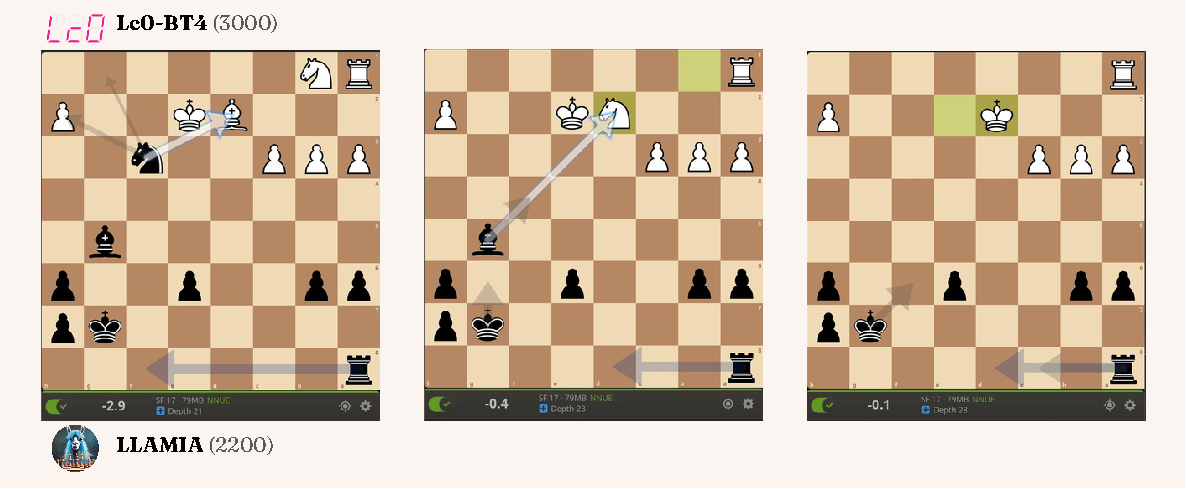
\includegraphics[width=0.95\linewidth]{tcp2.pdf}
    \caption{\textbf{Instruction Conditioned Planning:} LLAMIA is playing against an 800 higher-rated opponent. Note that played moves are indicated with white arrows, and the best moves are shown by blue arrows (size is ordered by the strength of the move). The following instruction is passed: ``your opponent is significantly weaker in endgames''. Orange and yellow moves indicate Mistakes and inaccuracies below. LLAMIA, in this position, plays the move \textbf{\textcolor{orange}{1... Nxd2??}} which is a mistake as it loses its advantage but creates a forced move sequence \textbf{[2. Nxd2 \textcolor{yellow}{Bxd2?} 3. Kxd2]} where it ends with a slightly better position in a rook endgame. Since our task design switches the Elo of Lc0 with a weaker policy here (1500) it ends up winning the game smoothly 19 moves later. LLAMIA was able to plan the forced exchange to trade down in an endgame where it knew it was better, demonstrating its superior planning. \textbf{FEN:[r7/6kp/pp2p2p/6b1/8/PPP2n2/3BK2P/RN6 b - - 0 1]}
}
    \vspace{-3mm}
    \label{fig:tcp}

\end{figure}

\label{app:conditional_planning_eval}
Players exhibit varying strategic strengths and weaknesses across different positional motifs, tactical patterns, and structural imbalances. To evaluate LLAMIA's ability to condition its policy on open-ended natural language directives—e.g., "target opponent’s endgame weaknesses"—we construct a benchmark to test LLAMIA’s ability to exploit such information when provided as a string.

We curate a set of 25 strategic motifs, selected based on: (a) their presence across all skill levels, (b) detectability via automated board heuristics or engine rollouts, and (c) coverage of diverse planning scenarios. Each motif category reflects a distinct type of strategic adaptation. We categorize them as follows:

\begin{enumerate}
    \item \textbf{Endgames:} Detected by material thresholds examples including.
    \begin{itemize}
        \item King and pawn vs. king
        \item Queen endgames
        \item Rook endgames
        \item Opposite-colored bishops
        \item Lucena and Philidor positions
        \item Minor piece vs. pawn endgames
    \end{itemize}
    
    \item \textbf{Pawn Structures:} Detected via relative pawn geometry:
    \begin{itemize}
        \item Isolated pawns
        \item Doubled pawns
        \item Backward pawns
        \item Passed pawns
        \item Pawn chains
        \item Hanging pawns
    \end{itemize}
    
    \item \textbf{Tactical Blunders:} Identified via engine rollouts revealing "only move" sequences leading to significant evaluation shifts (atleast a change of 400 centipawn evaluation):
    \begin{itemize}
        \item Knight Forks
        \item King Pins
        \item Overloaded defenders
        \item Mate in K$(K<5)$
        \item King Security
    \end{itemize}
    
    \item \textbf{Piece Coordination:} Defined via characteristic imbalances or pairwise dynamics:
    \begin{itemize}
        \item Two rooks vs. queen
        \item Knight and bishop vs. rook
        \item Queen and knight vs. queen and bishop
        \item Bishop pair vs. bishop and knight
        \item Rook on open file vs. unconnected rooks
    \end{itemize}
    
    \item \textbf{Repetition Traps:} Detected via rollout parsing for forced threefold repetitions
\end{enumerate}

Each game in the benchmark starts with an instruction (e.g. "Your opponent is signifcantly stronger than you, but has the following weakness ..., plan the moves to reach such positions to win even if it leads to a temporary disadvantage") and is played against a strong engine. If the model succeeds in steering the position toward the instructed motif, the engine is dynamically downgraded to a weaker engine. The win-rate differential serves as a proxy for strategic alignment and planning competence. The initial engine is Lc0-BT4 with search (>2500 ELO), if the weakness is reached we replace it with MAIA-1900 (emulates a 1900 Elo), note that LLAMIA's playing strength is $>2200$, essentially even at a significant disadvantage it can win over an engine rated more than 300 Elo lesser than it.

\begin{table*}[h]
    \centering
    \begin{adjustbox}{max width=1.05\textwidth}
    \begin{tabular}{c|ccccc|c}
    \toprule[1.2pt]
        \textbf{Model} 
        & \makecell{\textbf{End}\\\textbf{games}} 
        & \makecell{\textbf{Pawn}\\\textbf{Structures}} 
        & \makecell{\textbf{Tactical}\\\textbf{Blunders}} 
        & \makecell{\textbf{Piece}\\\textbf{Coordination}} 
        & \textbf{Repetition} 
        & \makecell{\textbf{Overall}\\\textbf{Improvement}} \\ 
    \midrule
        \textbf{ChessGPT-3B} 
        & 1\% & 1\% & 0\% & 0\% & 2\% 
        & 1.3\% \\
        \textbf{ChessGPT-7B} 
        & 2\% & 2\% & 1\% & 1\% & 3\% 
        & 2.5\% \\
        \textbf{ChessGPT-13B} 
        & 4\% & 4\% & 3\% & 3\% & 5\% 
        & 4.6\% \\\midrule
        \textbf{GPT-4o} 
        & 6\% & 7\% & 5\% & 4\% & 8\% 
        & 6.1\% \\
        \textbf{LLaMA-3.1 405B} 
        & 7\% & 8\% & 6\% & 5\% & 9\% 
        & 7.0\% \\
    \midrule
        \textbf{GPT-4o + Lc0 (Tool-Calling)} 
        & 10\% & 11\% & 9\% & 7\% & 12\% 
        & 9.2\% \\
        \textbf{LLaMA-3.1 405B + Lc0 (Tool-Calling)} 
        & \valgood{11.5\%} & 11.5\% & \valgood{11\%} & 7\% & \valgood{13\%} 
        & 10\% \\
    \midrule
        \textbf{LLAMIA-7B LoRA} 
        & 7\% & 8\% & 6\% & 5\% & 9\% 
        & 7.0\% \\
        \textbf{LLAMIA-7B} 
        & 11\% & \valgood{12\%} & 10\% & \valgood{8\%} & \valgood{13\%} 
        & \valgood{14\%} \\
        \textbf{LLAMIA-13B LoRA} 
        & 8\% & 9\% & 7\% & 6\% & 10\% 
        & 8.0\% \\
        \textbf{LLAMIA-13B} 
        & \valbest{17\%} & \valbest{19\%} & \valbest{14\%} & \valbest{11\%} & \valbest{20\%} 
        & \valbest{17\%} \\
    \bottomrule[1.2pt]
    \end{tabular}
    \end{adjustbox}
    \caption{
\textbf{LLAMIA-Bench Instruct-Conditioned Planning.}  
We evaluate whether models can adapt their strategy in response to explicit instructions about opponent weaknesses an ability crucial for flexible, human-aligned planning. This benchmark measures win-rate improvement when the model is informed that its opponent is vulnerable in specific areas, such as \emph{endgames}, \emph{pawn structure}, or \emph{tactical oversight}. Models play against a stronger engine; if they steer the game into the designated weakness domain, the engine is swapped with a weaker version, allowing the model to capitalize on its plan. While traditional engines (e.g., Stockfish, Lc0) remain invariant and show no improvement (0\%), and large tool-augmented models like GPT-4o + Lc0 achieve moderate gains (9–11\%), LLAMIA-13B delivers the strongest adaptation with a 16.2\% average win-rate gain across five weakness categories. Notably, smaller LoRA-adapted LLAMIA variants outperform much larger LLMs, demonstrating that internalizing structured planning signals via latent-state projection leads to more efficient and interpretable adaptation than external tool-calling or scale alone. Detailed evaluation setup is describe in \cref{app:conditional_planning_eval} \textbf{Overall Improvement} is the weighted average win rate over the subtasks. 
}

    \label{tab:instruct_conditioned_planning}
\end{table*}



% \begin{figure}[!h]
%     \centering
%     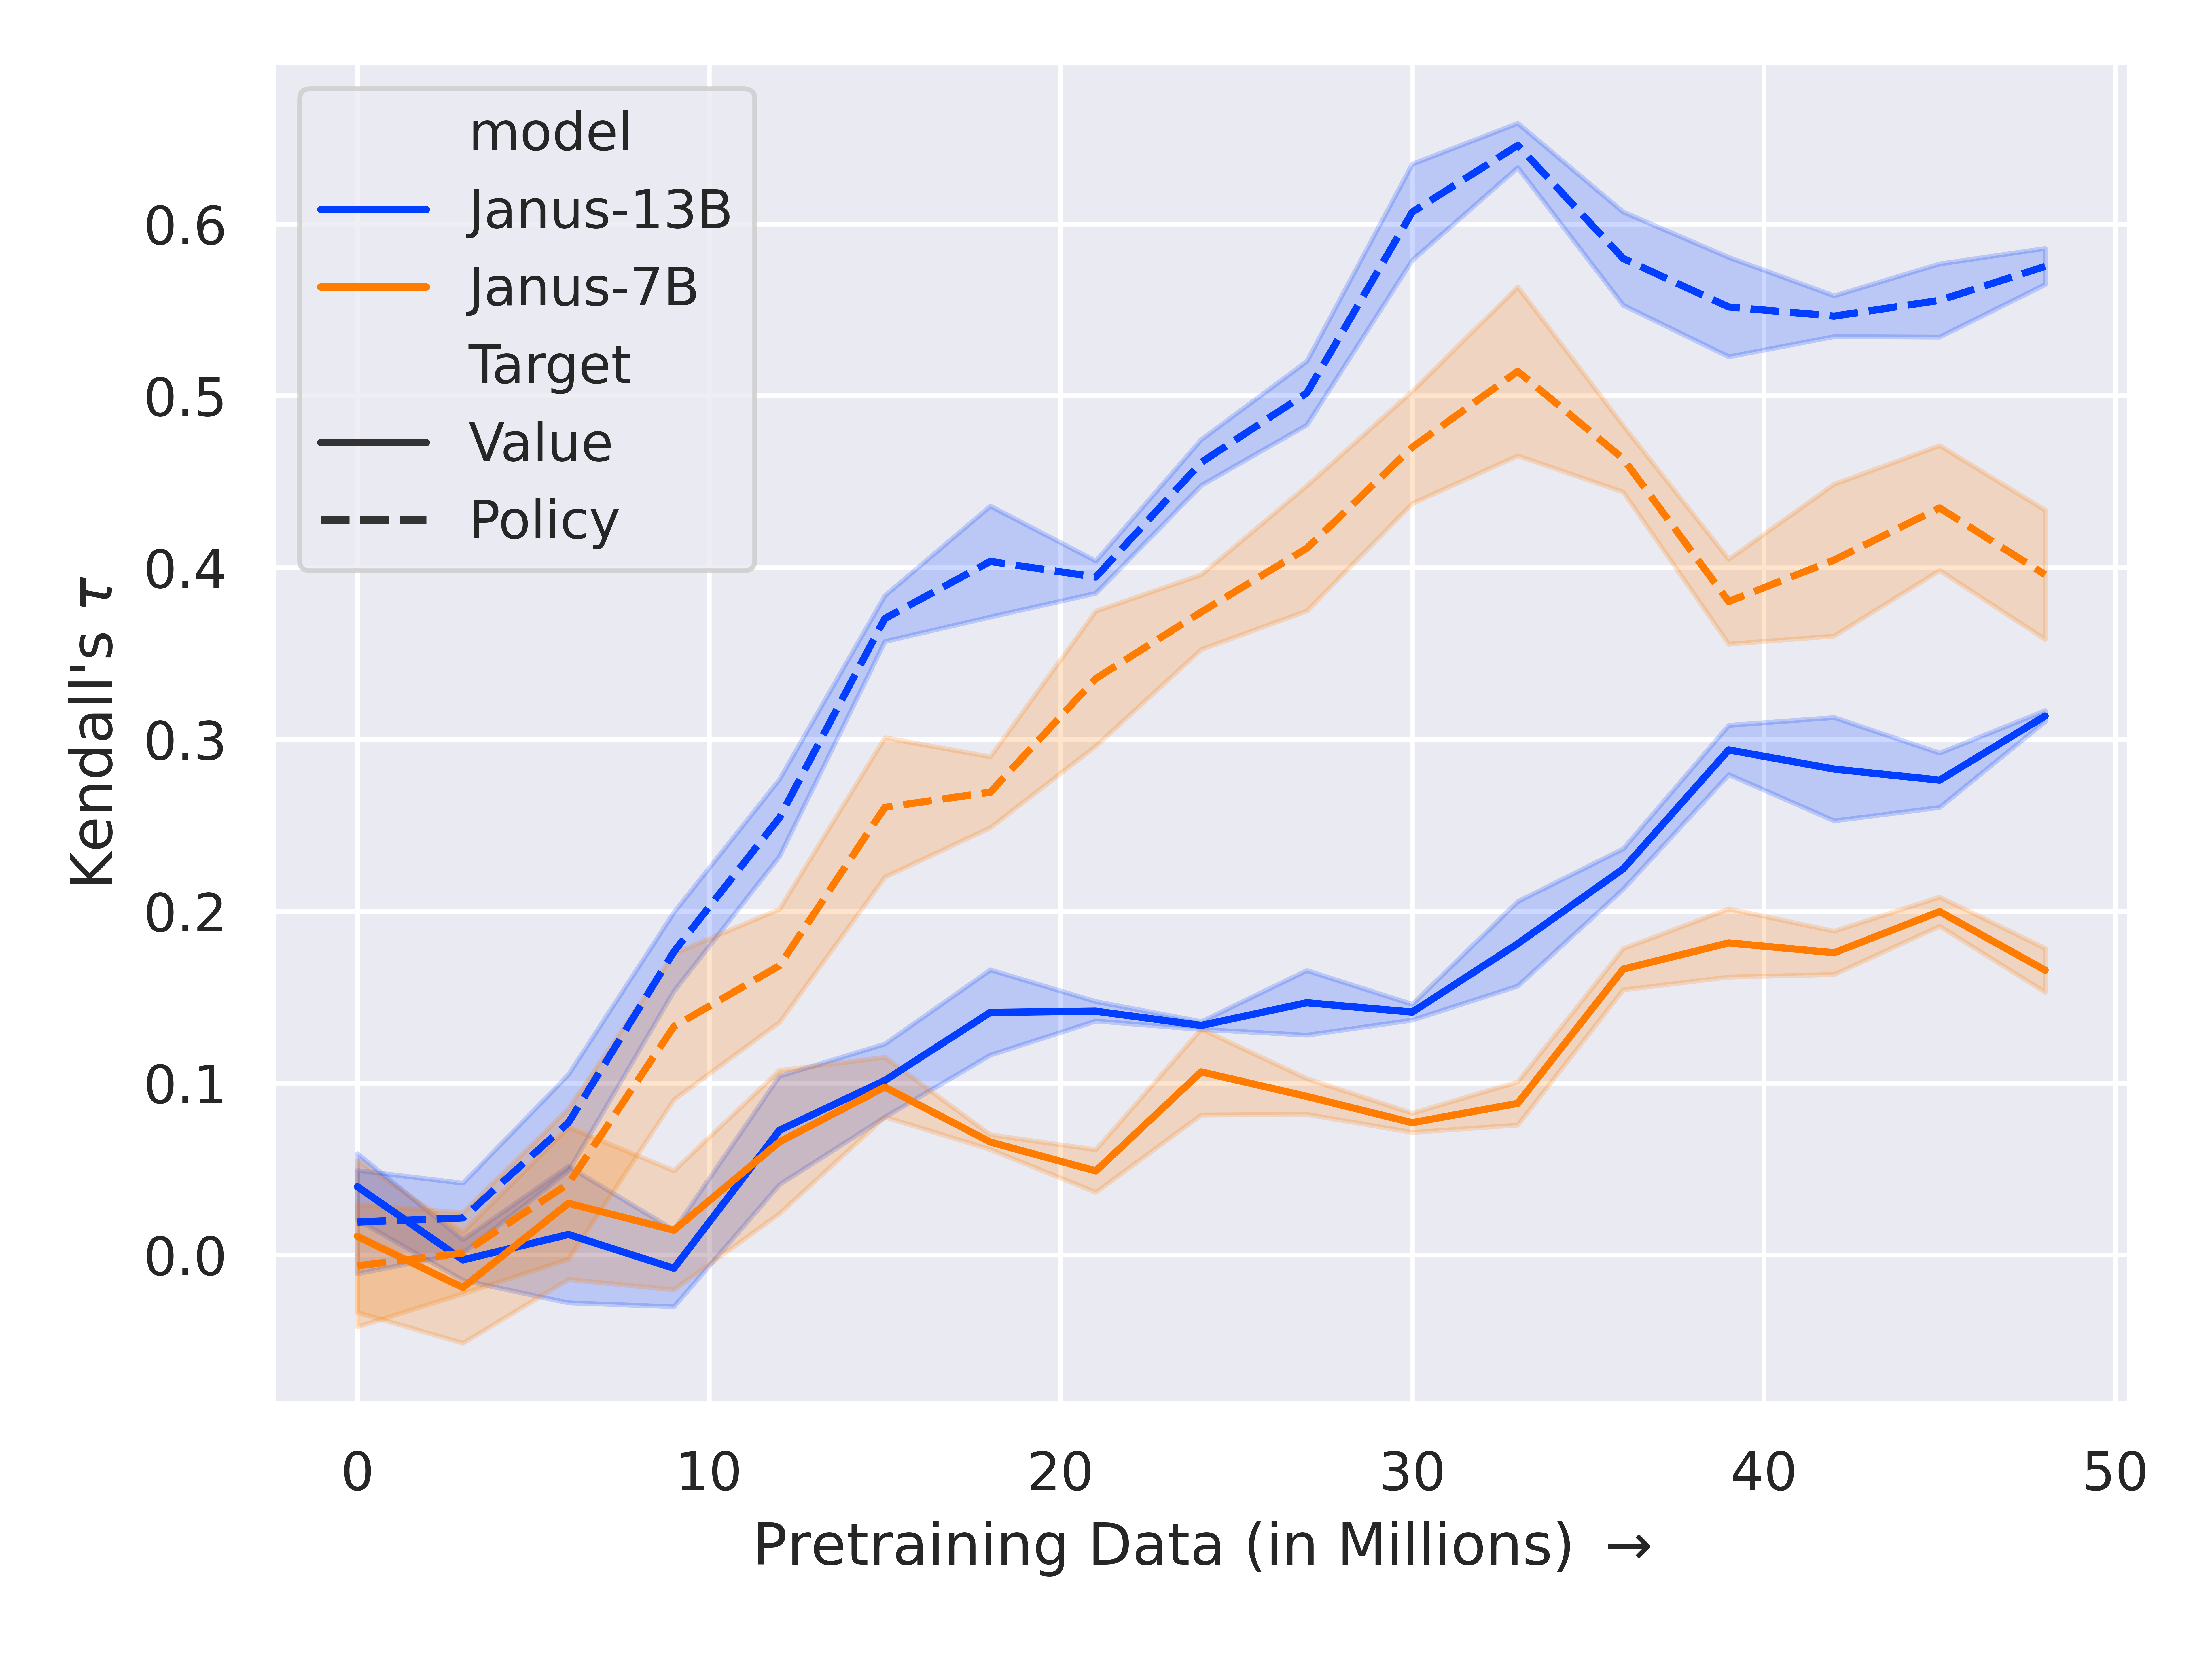
\includegraphics[width=\linewidth]{KendalTau_Alignment.png}
%     \vspace{-8mm}
%     \caption{\textbf{Kendall-$\tau$ alignment} scaling with data and parameters. The alignment between the LLM's policy and Agent's Value (Q-values post search) and Policy (Base policy). Over 30 million points the alignment with both policy and value improves, interestingly both 13B and 7B models exhibit an area (30M-40M) where they start deviating from policy to value, we call this the shallow ``internal search''}.
%     \label{fig:pretraining-curve}
% \end{figure}
\subsection{Environment Extension}
To evaluate the extensibility of our framework we extend our approach to two new tasks, \textbf{Text-to-Image Preference Alignment} to predict and improve alignment of image generation models and goal directed language through \textbf{PersuasionBench}. We follow the exact same setup, training data, and evaluation protocol as \cite{xu2025visionrewardfinegrainedmultidimensionalhuman} and \cite{singh2024measuring}.






\begin{figure}[!h]
    \centering
    \includegraphics[width=\linewidth]{aesth (2).pdf}
    \vspace{-2mm}
    \caption{
\textbf{Qualitative Examples: Image Preference Alignment via Internalized Rewards.}  
We compare images generated using VisionReward (left), LLAMIA-ImageReward (middle), and human-preferred selections (right) across diverse prompts involving aesthetic composition, product photography, and stylistic variation. LLAMIA-ImageReward yields more coherent framing, superior lighting consistency, and better adherence to prompt-specific constraints, as also reflected in human preference studies (+5 pp). Notably, these improvements emerge with half the fine-tuning data, demonstrating LLAMIA’s capacity to internalize domain-specific reward functions and generalize stylistic priors across prompts.
}.
    \label{fig:image_grid}
\end{figure}
\FloatBarrier

\begin{figure}[htbp]
    \centering
    \begin{subfigure}[b]{0.5\linewidth}
        \centering
        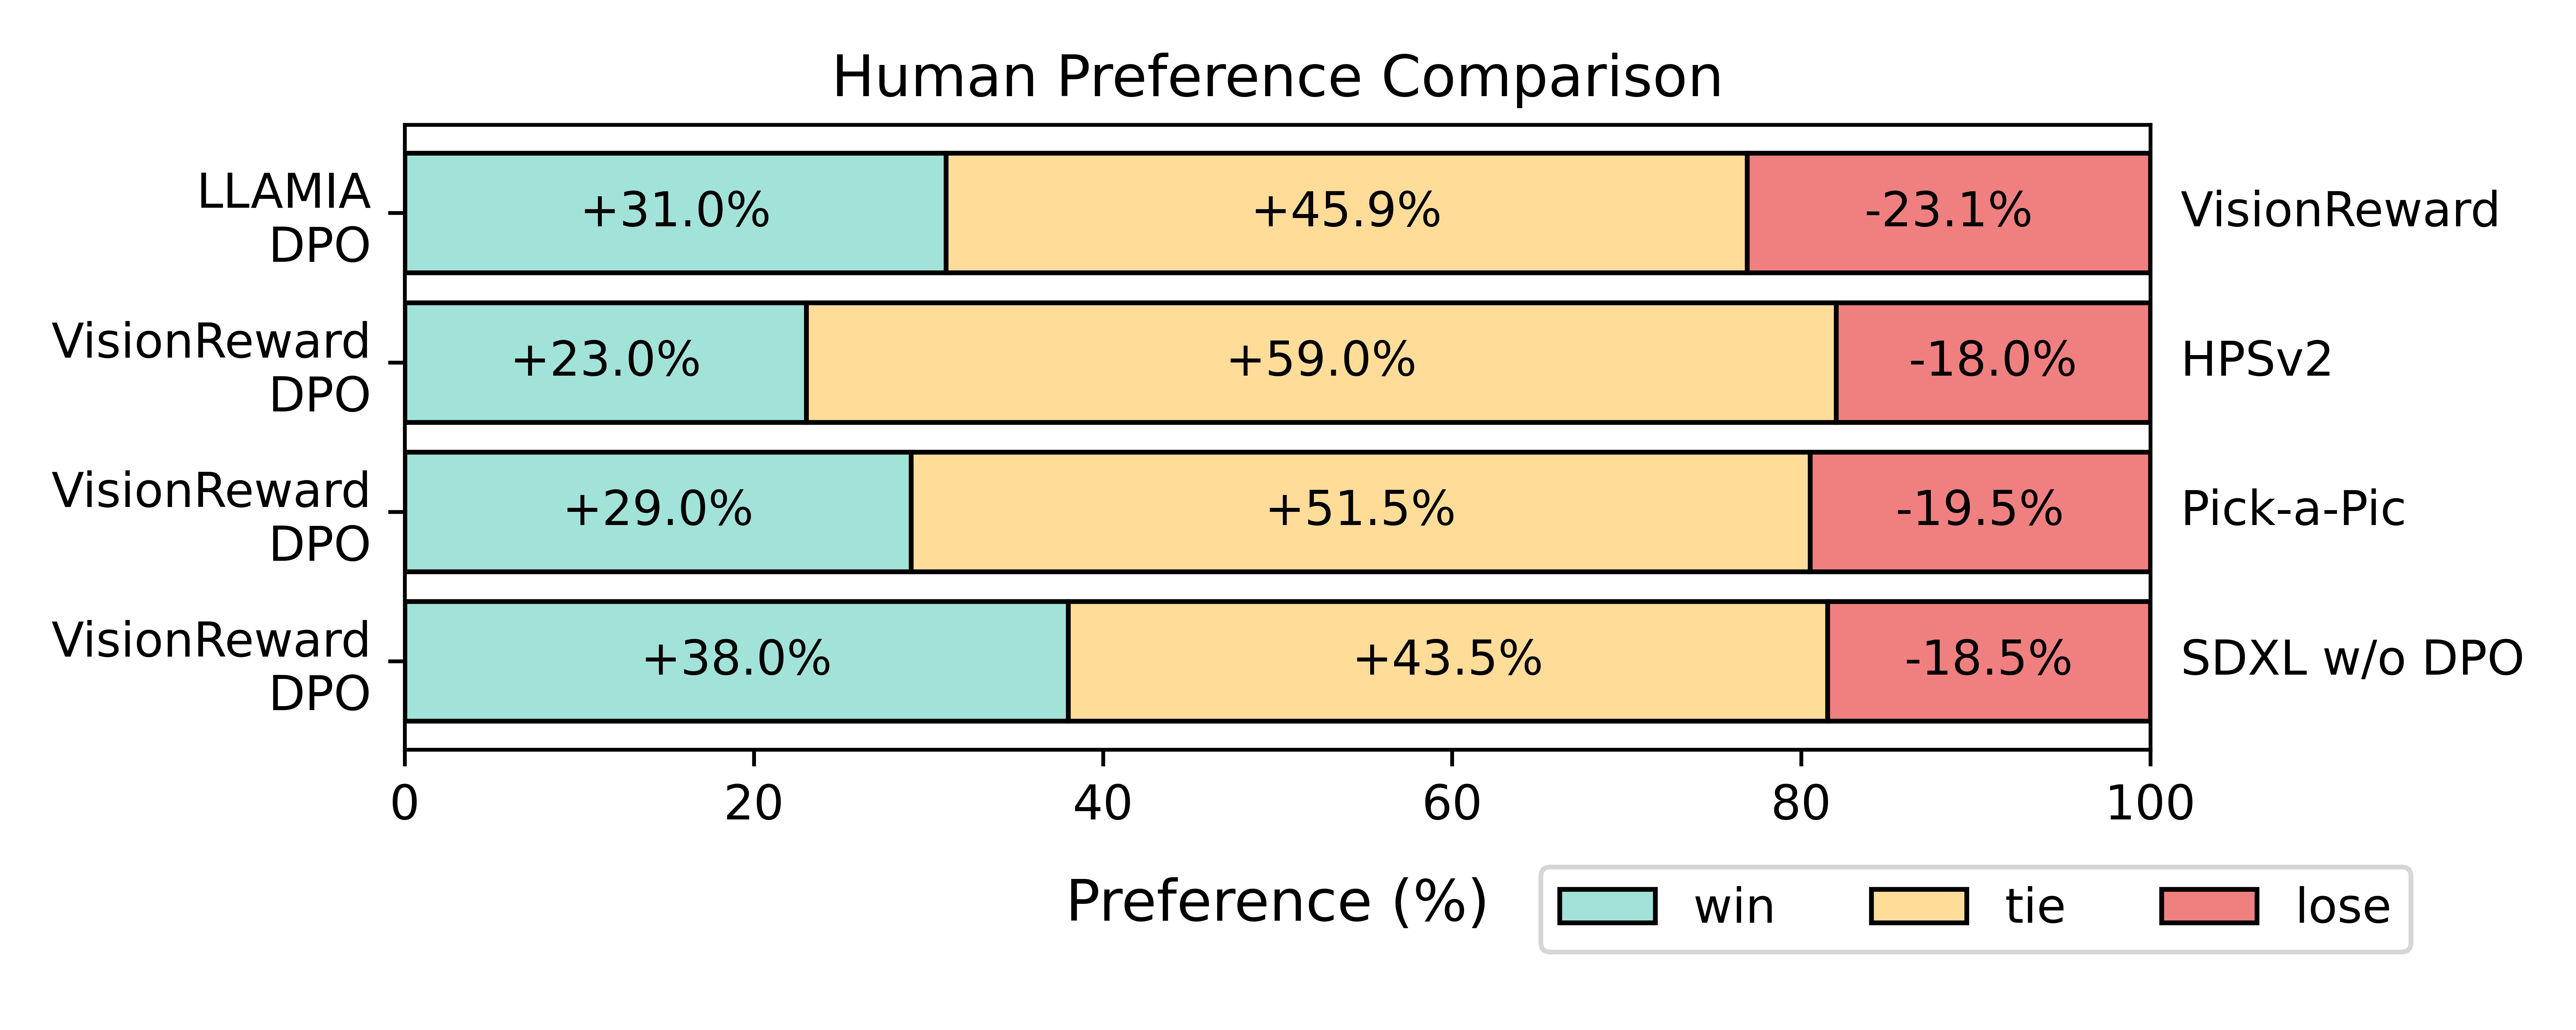
\includegraphics[width=\linewidth]{human_preference_comparison.png}
        \caption{\textbf{Human Preference Comparison:} Human raters prefer LLAMIA’s SDXL generations over VisionReward’s by a margin of +7.9\%. While VisionReward improves significantly over raw SDXL (e.g., +19.5\% win rate), LLAMIA’s internal reward alignment improves sample-level aesthetics and relevance further, as reflected in Pick-a-Pic and HPSv2 gains.}
        \label{fig:subfig-human-preference}
    \end{subfigure}
    \hfill
    \begin{subfigure}[b]{0.48\linewidth}
        \centering
        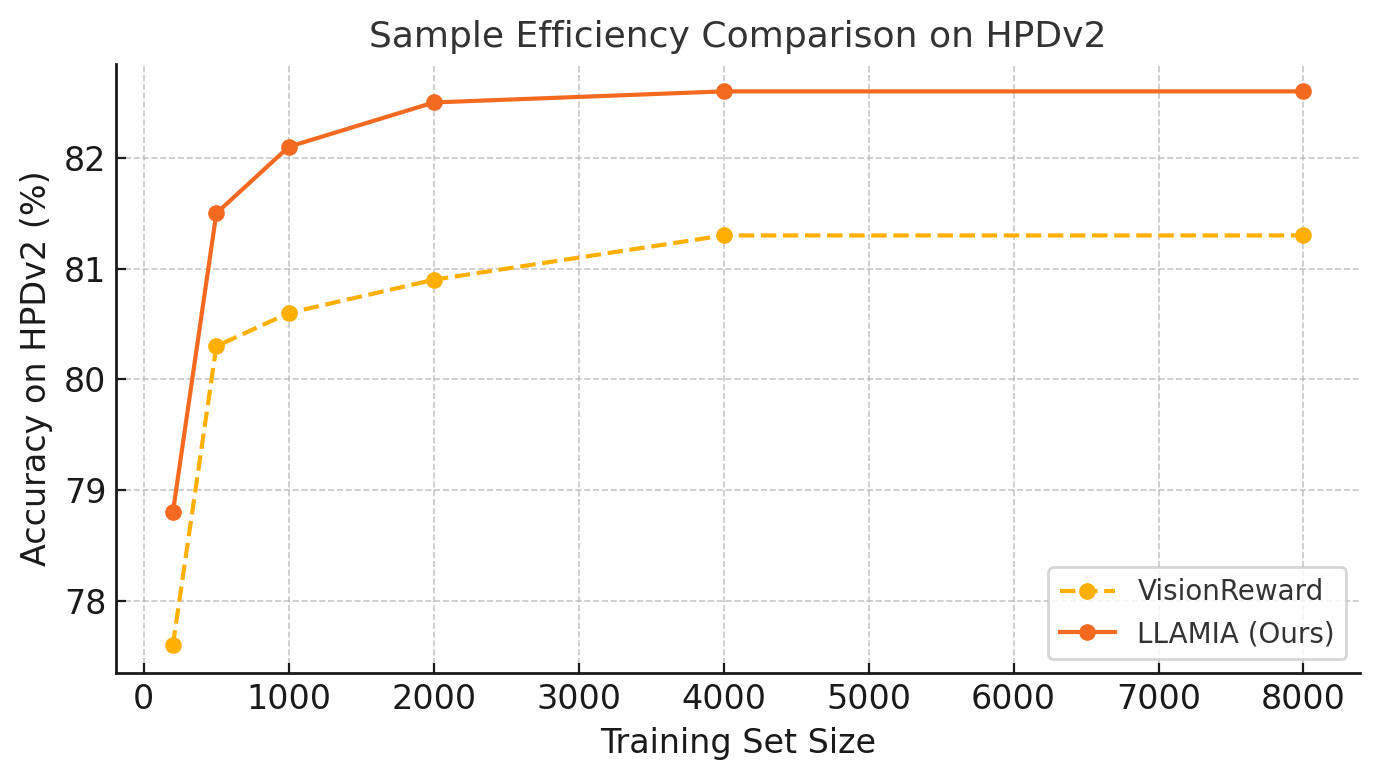
\includegraphics[width=\linewidth]{output (7).png}
        \caption{\textbf{Sample Efficiency on HPDv2:} LLAMIA shows significantly better sample efficiency over VisionReward on the HPDv2 benchmark. It achieves 81.3\% accuracy with just 2k samples, matching VisionReward’s peak accuracy with 8k samples. This highlights that internalizing ImageReward within the generation process yields more data-efficient preference modeling.}
        \label{fig:subfig-model-output}
    \end{subfigure}
\caption{\textbf{Quantitative Analysis of Visual Reward Alignment.} We compare LLAMIA to VisionReward across two axes: (a) sample efficiency of preference prediction and (b) human preference studies on DPO-enhanced SDXL generations. LLAMIA consistently achieves higher accuracy and win rates with fewer samples.}
    \label{fig:comparison}
\end{figure}

\clearpage

\section{Hyperparamaters}
\label{sec:hyperparams}
LLAMIA models (7B, 13B) were trained on five nodes of 80GB A100 GPUs, totaling
approximately eight days of computational budget.


\begin{enumerate}
  \item \textbf{Model Architecture}
  \begin{itemize}
    \item Backbone LLM: \texttt{lmsys/vicuna-13b-v1.5}
    \item Agent Model: \texttt{Lc0-BT4}
    \item Hidden size (LLM): 5120
    \item Agent encoder dimension: 1024
    \item Number of agent encoders: 15
    \item Number of LLM state tokens: 16
    \item Number of agent state tokens: 64
    \item Projector type: \texttt{SimpleMLP}
    \item Projector hidden dimension: 2048
    \item Projector hidden depth: 3
    \item Projector dropout: 0.1
    \item Projection layer: \texttt{encoder[\textbackslash d]+/ln2}
    \item Use state patch token: \texttt{true}
    \item Freeze LLM backbone: \texttt{true}
  \end{itemize}

  \item \textbf{Training Configuration}
  \begin{itemize}
    \item Number of epochs: 1
    \item Per-device train batch size: 70
    \item Per-device eval batch size: 32
    \item Learning rate: 6e-5
    \item Optimizer: AdamW (\(\beta_1 = 0.9, \beta_2 = 0.999, \epsilon = 10^{-8}\))
    \item Max gradient norm: 1
    \item Scheduler: Cosine
    \item Warmup ratio: 0.05
    \item Gradient accumulation steps: 1
    \item Gradient checkpointing: \texttt{true}
    \item Mixed precision: bfloat16 
    \item Quantization: \texttt{nf4}
    \item Double quantization: \texttt{true}
    \item Deepspeed config: Deepspeed Zero2 with Offload
  \end{itemize}

\end{enumerate}


\section{Paper rewrite items}
Neurips
\begin{itemize}
    \item variables unclear in eqn1
    \item 
    
    
\end{itemize}



% This document was modified from the file originally made available by
% Pat Langley and Andrea Danyluk for ICML-2K. This version was created
% by Iain Murray in 2018, and modified by Alexandre Bouchard in
% 2019 and 2021 and by Csaba Szepesvari, Gang Niu and Sivan Sabato in 2022.
% Modified again in 2023 and 2024 by Sivan Sabato and Jonathan Scarlett.
% Previous contributors include Dan Roy, Lise Getoor and Tobias
% Scheffer, which was slightly modified from the 2010 version by
% Thorsten Joachims & Johannes Fuernkranz, slightly modified from the
% 2009 version by Kiri Wagstaff and Sam Roweis's 2008 version, which is
% slightly modified from Prasad Tadepalli's 2007 version which is a
% lightly changed version of the previous year's version by Andrew
% Moore, which was in turn edited from those of Kristian Kersting and
% Codrina Lauth. Alex Smola contributed to the algorithmic style files.
\begin{comment}
    \section{Feedback}
Continous vs Discrete

\begin{enumerate}
    \item What defines a foundational model?
    \begin{enumerate}
        \item (Bommasani et al. 2021). Foundation models constitute large-scale AI models that are pre-trained on vast amounts of general data and that can be adapted for downstream applications (e.g., by fine-tuning them through further training on application-specific data). Through this pre-train and adapt approach they expedite the development of innovative AI products and services and accelerate the accessibility of high-performance AI solutions in various industries (Teubner et al. 2023).
        \item With scaling, foundation models are becoming increasingly good at performing tasks they were not explicitly trained for, thereby broadening the scope of applications achievable by a single model without the need for additional training data or fine-tuning (Brown et al. 2020).When needed, task-specific performance can be further enhanced through fine-tuning or effective prompt engineering techniques; (Liu et al. 2023; Niu et al. 2020).
        \item Following Bommasani et al. (2021, p. 1), we define a foundation model as ``any model that is trained on broad data that can be adapted to a wide range of downstream tasks''. Through this combination of task-agnostic pre-training and subsequent fine-tuning, foundation models enable new approaches to building and deploying AI systems.
        \item Emergent Capabilities The first key feature of foundation models is the emergence of behavioral capabilities that were not explicitly constructed, nor expected, by human developers, which frequently is referred to as in-context learning (Min et al. 2022)
        \item \cite{XXXFlava} a true foundation model in the vision and language space should not only be good at vision, or language, or vision-and language problems–it should be good at all three, at the same time.
    \end{enumerate}
    \item What would characterize a foundational decision model
    \item What constitutes an FDM
    \item Why Chess
    \somesh{P2 @Harini ChessFormer, AlphaZero}
    \begin{itemize}
        \item 
    \end{itemize}
    \item Emergent Properties across Large Decision Models
    \item Why search or runtime compute
    \item Why Language and Decisions
    
\end{enumerate}








Planning is a key task in real-world scenarios whiuch has not been solved in the generality needed by any foundation models [cite: Yann Le Cun tweeted a reference for this]. 

Foundation models for decision making should look like... creation of adapters - one per environment. We provide one approach - RLQA to create foundation models for decision making.

Task specific specialist models have their own disadvantages such as limited generalizability. To get the best of these two approaches, researchers have proposed coupling LLMs with specialist policies using toolformers, agentic models etc. [cite: ].



However, this loose coupling cannot solve tasks which require the LLM to understand the specialist policy. Some concrete examples of such tasks include commentary generation in games, language conditioned policy adaptation, language based behavior generalization etc. To bridge this gap, we propose an approach called RLQA, where we tightly couple the LLM and the specialist policy using a policy-language adapter. In this paper, we present an approach to train this adapter, provide benchmarks to test the efficacy of the coupled LLM and specialist policy and provide demonstrations of tasks where our RLQA approach significantly outperforms other popular approaches in literature either in terms of accuracy or efficiency. In this paper, we restrict attention to chess, but our approach is extensible to any planning problem in general.

Fig-1 with descriptive caption - inference pipeline
One paragraph on approach and motivation, novel tasks, datasets and benchmarks


Generalist agent for a single environment - can generate/simulate multiple behaviors in a text controlled manner. A method to align an agent and an LLM a foundation model in decision making and decision understanding
Emergent properties on unseen tasks
Bridging the gap between specialized agents and LLMs via our own connectors:
1. to solve greater tasks which cannot be solved by these independently or weakly coupled
2. example commentary generation, fine-tuned behavior cloning, conditional decision making - example opponent/environment conditioning


Contributions need to be differentiated - Benchmark vs Algorithm vs Model \somesh{1 Algorithm, 3 Datasets, 4 Benchmarks How should we do this?}

Benchmark: Are we providing an arena for testing other RL agents? \somesh{Yes}


Effectiveness of Generalized Decision Making - needs to be defined... \somesh{Conditional Decision Making - Similar to Behavior, Explanation - Directly state annotation, game analysis. Agent identification- Cheating Detection, Improving search - LLMCTS :P}

\begin{enumerate}
    \item What is a foundational model ? A foundation model is any
model that is trained on broad data (generally using self-supervision at scale) that can be adapted (e.g., fine-tuned) to a wide range of downstream tasks; current examples include BERT [Devlin et al.2019], GPT-3 [Brown et al. 2020], and CLIP [Radford et al. 2021]
\end{enumerate}

\somesh{What to capture: What does a foundational decision making model need, an LLM and a policy or representation learning model, and a generalized method to connect these. What should it be trained on? Large Unsupervised number of decisions, and rewards/evaluation.}
\subsection{Contribution}
1. Foundation Decision models
    1.1 Behaviour cloning in few shots, or IFT with 10\% of the data, one model vs finetunes.  Table 1
    1.2 Behaviour stylometry: Unseen task, Comparable or better results with, 15\% of  shots across 20,40,112,High Ranked, GMs, Bots, Elo identification, Time formats table 1.3 
2. We are able to get the strongest known raw policy 
https://arxiv.org/pdf/2402.04494

2. Comparison against Llama3.1 405B with tool calling to Lc0 + MCTS, and GPT-4o with Evaluation and next best moves from Lc0 + MCTS. (All tables) Projection tokens in FDM perform better than tool calling on more than 30x larger LLMs. (All tables)

3. What can an FDM do? Results breakdown why are FDMs needed
    1. Only LLM tasks: position description
    2. Only Engine tasks: puzzle
    4. One model to all
    3. Neither finetune nor agentic task: commentary, position difficulty, rating,
Breadth of tasks with the star-graph

4. What data goes into an FDM:
    1. Self-supervised large scale data (Existing positions and their evals)
    2. Demonstrations from humans (BC)
    3. Complex Instruction data (small scale, downstream applications)

5. Results and analysis
Appendix Lucena

6. Extend this to other envs.


OPenreview
1. Towards building a foundation decision model



4. Commentary generation, 

5. Decision Understanding
https://aclanthology.org/P18-1154.pdf
https://aclanthology.org/P19-1597.pdf
https://arxiv.org/pdf/2212.08195
5. Emergent Abilities unlocked via jointly training with agent projections: Breadth of tasks
6. Towards fdm ?

1. Using Decisions or Policy as a modality unlocks downstream capabilities. (LLaVA sense - DT is an input as opposed to a competition)
    Relevant Results:
        a. State Value Multi Choice, Annotation, Commentary, BOT classification, Puzzles Understanding, Game Masking
        b. Downstream capabilities such as game or
state commentary generation, we outperform SOTA models and even upto 10x larger LLMs
assisted with super-human engines

2. LLMs with Optimal Policy are effecient 0-shot behavior cloners (simulators)
    a. Behavior cloning all results

3. LLMs are strong and efficient look ahead models
    3.1 LLMs themselves model N-step lookahead better than agent trained on that task (Performance, Data required)
    3.2 LLMs that learn look ahead modelling improve downstream performance (tasks)

4. 
\section{Learning to Look Ahead}
Any problem that requires planning can be described by

\begin{enumerate}
    \item A problem statement or current state (S)
    \item A proposed solution or Action (A)
    \item Approximate feedback (F)
    \item An agent or policy (P) that can generate sub-optimal or near-optimal actions.
\end{enumerate}
Current research solves this task by using (P) obtained from self-supervised learning on large amounts of data, as a heuristic to do a "search", or a chain of intermediate actions, which progressively lead to $max(F)$. The resulting search, the tree of actions, is able to solve the problem statement better.

In this work we try to answer the following questions

\begin{enumerate}
    \item Can LLMs exploit an agent's heuristic to plan N-step ahead? We know that Lc0's NN has a policy of only 2600, + MCTS 3500
    \somesh{Note to self: For general problems the LLM itself is the agent}
    \begin{enumerate}
        \item We further train the agent to predict the optimal actions -> +21
        \item We train RLQA to predict the optimal actions -> +53
        \item We train RLQA to predict the optimal actions and the chain-of-thought (the best path in the tree of actions) to it -> +143
    \end{enumerate}

    \item What is the value of the explicit search (
\end{enumerate}
1. Can LLMs exploit an agent's heuristic to plan N-step ahead?
    1.1. We train an agent to predict the optimal policy -> +21
    1.2. We train Agent+LLM to predict the optimal policy -> +53
    1.3. (Train-time) We train Agent+LLM to predict the ToT + optimal policy -> +143 -> Input: FEN(Board) -> Output: Evaluation and next best moves until 30 depth (3500 Elo)
    1.4. (Train-time) We train Agent+LLM to predict the ToT + optimal policy -> +143 -> 
        Input: FEN(Board)
        Output: Evaluation + (next best moves + environment verbalization) until 30 depth (3500 Elo)
        Ablations 1. Only ground truth 2. Synthetic w Ground truth (Agadmator vs Crowd sourced vs Random Tokens)
    1.5. (Train-time) We train Agent+LLM to predict the ToT + optimal policy -> +143 -> 
        Input: FEN(Board)
        Output: Evaluation + (next best moves + annotation/commentary) until 30 depth (3500 Elo)
    1.6. (Train-time) We train Agent+LLM to predict the ToT + optimal policy -> +143 -> 
        Input: FEN(Board)
        Output: Evaluation + (next best moves) until 30 depth (3500 Elo) + Commentary/Annotation of the 3500 Elo
    1.7. (Game-level commentary) We train Agent+LLM to predict the ToT + optimal policy -> +143 -> 
        Input: FEN(Board)
        Output: Evaluation + (next best moves) until 30 depth (3500 Elo) + Commentary of the 3500 Elo
    
2. What is the value of the explicit search tokens?
    2.1. We train an agent to predict the (ToT + optimal policy), Infer w/o ToT -> +76

3. How can we train an LLM to plan with progressive Tree of thoughts
    3.1 We IFT the optimal path and pruning -> +36
    3.2 We IFT the optimal path and pruning progressively -> +75
        Input -> FEN
        Output -> Eval + Next-best move

O1 analogy, 


Parameter Count Trend
1. Concluding that what may not work for smaller models may not translate to stronger models

\section{Model}
\emph{Getting representations from an expert engine, adapting it and then feeding the adapted representation to an LLM to do the following downstream tasks - multi-choice chess annotation, checkmate puzzles, state-value multi-choice, encoding <--> PGN (verbalization) bidrectional; need to check if adding the encoding helps at all, \textbf{behavior simulation (ACM 2018, Maia Chess) - one model, multiple Elos (and also one specific player), accuracy, commentary generation (beating SOTA based on state-level commentary generation - we will do trajectory-level)}}

We consider the standard MDP based RL framework with the usual notation. Let $\pi^*$ denote a learnt (optimal) policy using any RL based approach that also yields $Q^*$, the optimal state-action values. We then look at the following problems:
\begin{enumerate}
    \item Policy Explanation: Given $\pi^*$, $Q^*$, the corresponding state space $\mathcal{S}$ and a state featurizer (could be a textual featurizer), we create a dataset $\widehat{\mathcal{D}}$ of $\{(S_t, f_t, A_t, Q_t,)_{t=0}^T \}_{i \in \mathcal{D}}$, where:
    \begin{enumerate}
        \item $i$ represent an episode from $\mathcal{D}$ which is an offline (can be batch or online as well) dataset of episodes/trajectories.
        \item $t \in \{0, T\}$ represents the step in the episode.
        \item $S_t \in \mathcal{S}$ represents the state at time $t$.
        \item $f_t$ represents the verbalized features of $S_t$.
        \item $A_t \sim \pi^*(S_t)$ represents the action chosen at time $t$ using policy $\pi^*$.
        \item $Q_t = Q^*(S_t, A_t)$ represents the action-value starting from state $S_t$ and choosing action $A_t$.
    \end{enumerate}
    Using this dataset, $\widehat{\mathcal{D}}$, as a first task, we finetune an LLM to predict the $Q$ values given the rest of the sequence. For the purpose of this experiment, we consider the following potential list of environments:
    \label{ref:Candidate envs for text}
    \begin{enumerate}
        \item \url{https://github.com/carla-simulator/carla}
        \item \url{https://github.com/microsoft/TextWorld}
        \item \url{https://github.com/ronentk/TextLabs}
        \item \url{https://github.com/IBM/visual-hints-textworld-rl}
        \item \url{https://github.com/google-deepmind/open_spiel}
        \item \url{https://github.com/Farama-Foundation/Minigrid}
        \item \url{https://github.com/allenai/ScienceWorld}
        \item \url{https://github.com/fidler-lab/social-driving}
        \item \url{https://github.com/google-deepmind/android_env}
        \item \url{https://github.com/facebookresearch/nocturne}
        \item \url{https://github.com/microsoft/CyberBattleSim}
    \end{enumerate}
\end{enumerate}

10M games existing
600B positions pre-existing SF-16

No. of possible positons >>> 600B positions pre-existing SF-16

Twitter:

Dataset: -> Low time
Agent -> Time series
Training -> Low time
Evaluations -> Transsuasion time



\section{Extension}
\subsection{Video Planning}
For long videos LLMs are used to generate video plans, \cite{VideoStudio,DirectorGPT} we will generate multi scene ads, we will plan it with FDM .

1. Optimal Decision making -> Ad Plan Generation from title, intent
2. Conditional Decision making -> Ad Plan generation given scene, conditions etc.
3. GDU/Commentary: Explain a scene (describe, 

1. Decision Making -> Video Plan Generation (memorable, likes/views)
2. Generalised Decision Making (Scene Fill / Complete) -> Behaviour Cloning (GDM)
3. -> Decision Understanding
\subsection{MultiGame DT}

\newpage
SFT: Transsuasion [Vicuna(13B)]: 0.31
Agent: Chronos-base (univariate): 0.09
Agent: Chronos-base (self+industry): 0.17
Pretrain: LLAMIA[Vicuna(13B) + Chronos-base (self+industry)]: 0.28
Pretrain+SFT: LLAMIA[Vicuna(13B) + Chronos-base (self+industry)]: 0.49

\somesh{Qualitative analysis of what LLM learnt from TS agent}
\somesh{Add LLM hidden state into chronos embedding}
LLM Learnt Optimal Policy:



LLAM:
    Input:
        Board position embedding + FEN 

    Output:
        (+7.2) Moves: m1 m2 m3 m4
        Also PV1: 6.1 m1, m2, m3


Finetuned Vicuna:
    Input:
        Board FEN, SV, Evaluation is (+7.2) on move m1

    Output: 
        m2 m3 m4
\begin{figure}[!h]
    \centering
    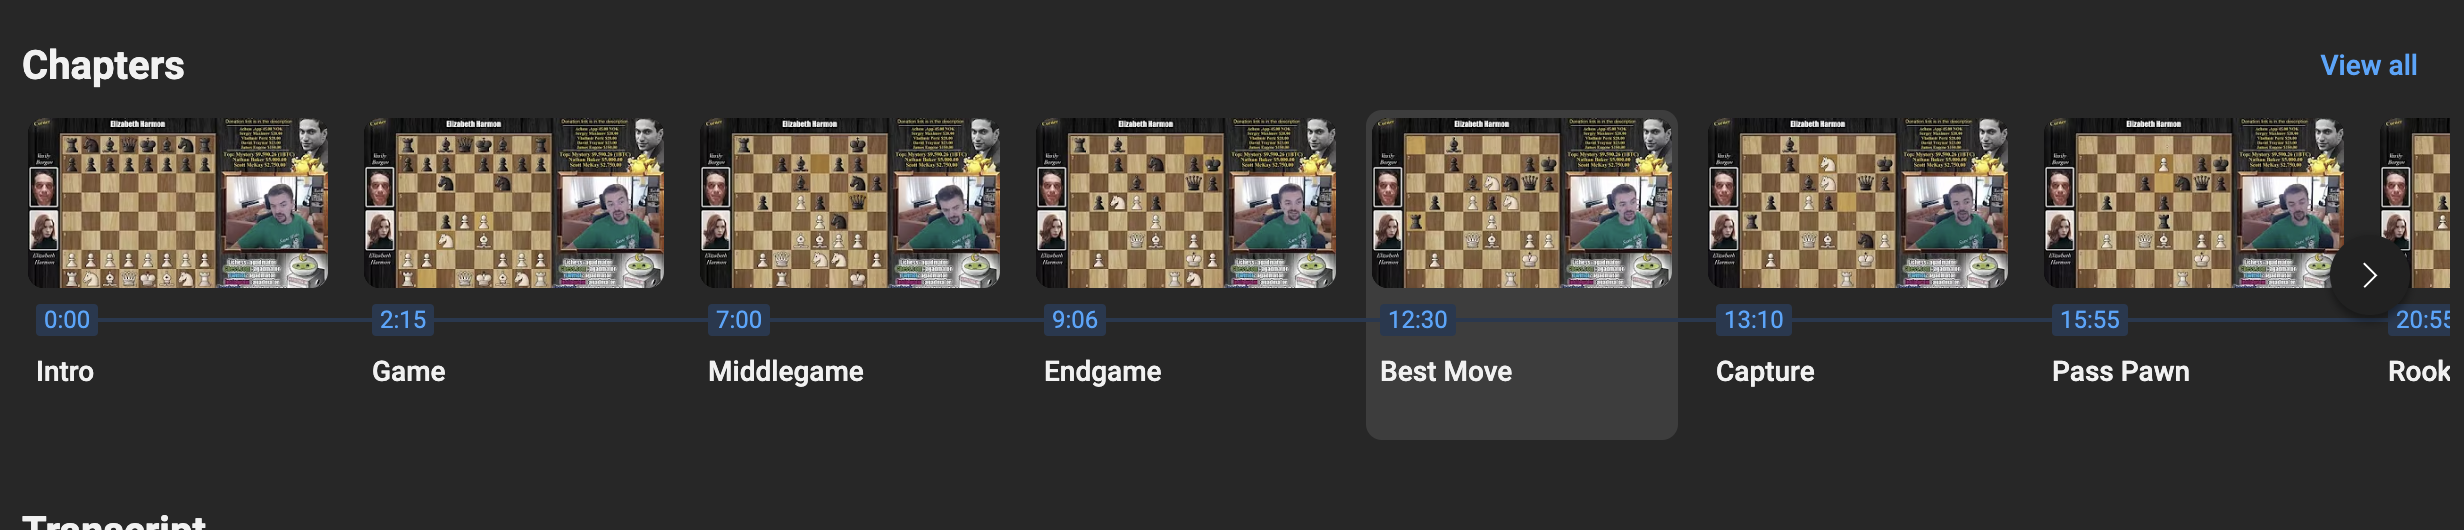
\includegraphics[width=\linewidth]{Screenshot 2025-01-22 at 5.18.04 PM.png}
    \caption{Game Commentary: Qualitative game segments annotated, with panel wise transcripts, compared with actual and GPT-4o}
    \label{fig:enter-label}
\end{figure}

\begin{figure}[!h]
     \centering
     \begin{subfigure}{0.45\textwidth}
         \centering
         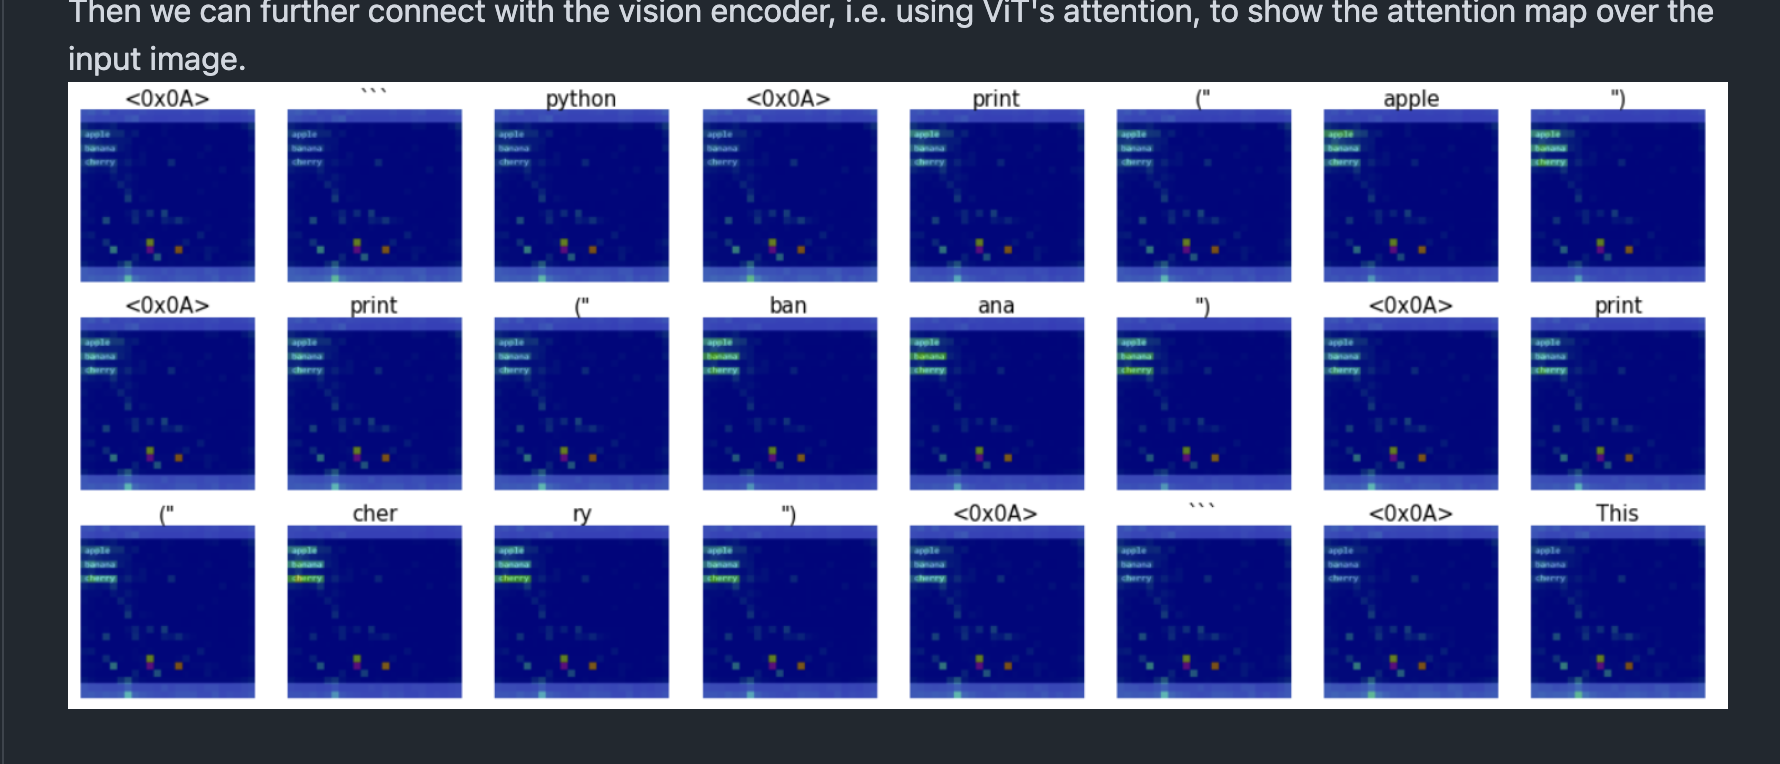
\includegraphics[width=\linewidth]{Screenshot 2025-01-22 at 5.46.55 PM.png}
         \label{fig:1a}
     \end{subfigure}
     \begin{subfigure}{0.45\textwidth}
         \centering
         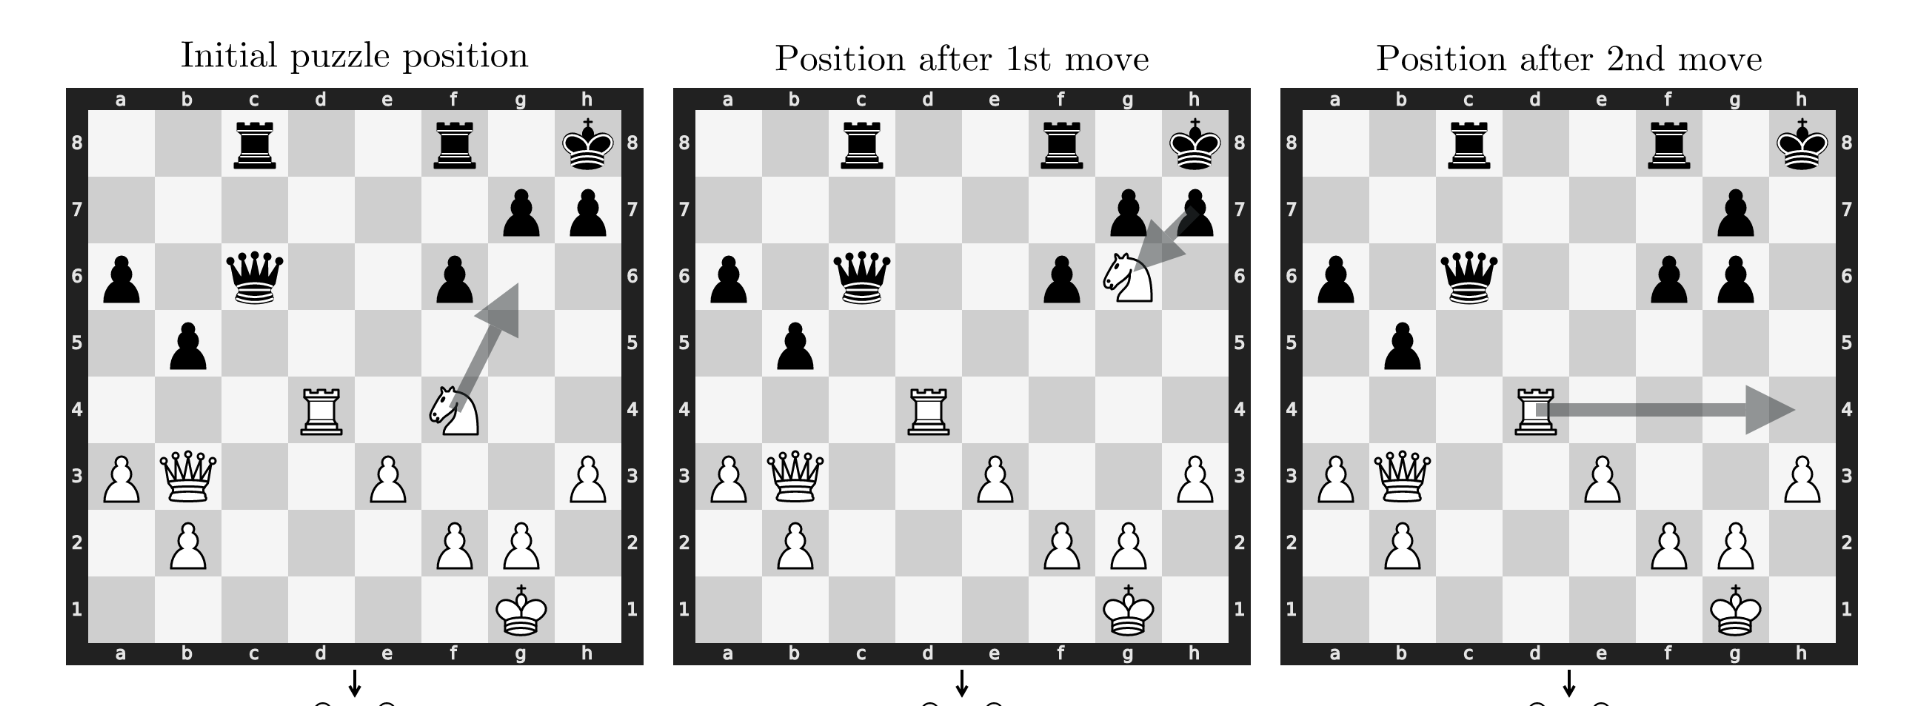
\includegraphics[width=\linewidth]{Screenshot 2025-01-22 at 5.50.06 PM.png}
         \label{fig:1b}
     \end{subfigure}
     \caption{Attention Visualization of board from decision tokens with different instruction on a position}
     \label{fig:1}
\end{figure}

\begin{figure}[!h]
    \centering
    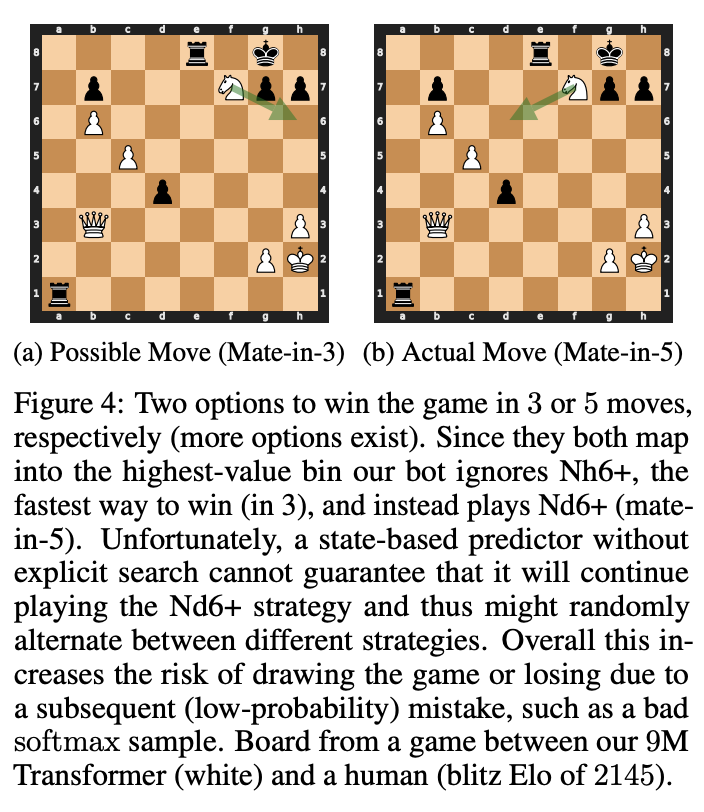
\includegraphics[width=\linewidth]{Screenshot 2025-01-22 at 5.39.44 PM.png}
    \caption{Move by move comparison on different BCL cases (Elo, DeltaElo, Time, Format)}
    \label{fig:enter-label}
\end{figure}

\subsubsection{Commentary}
We collect data of commentary on chess games from a famous Youtube channel called Agadmator aka Antonio Radić. On his channel, Radić reviews recent tournament games from top players, historical matches, and chess compositions. Almost all of Radić's videos follow the same format: a detailed analysis of one chess game. We extract paired commentary from the transcripts by aligning video clips with natural language transcripts based on timestamps.
\end{comment}

% \section{Introduction}
% \vspace{-2mm}

% % =============================================================================
% % PARAGRAPH 1: What is the problem?
% % =============================================================================

% Large language models excel at tasks solvable through next-token prediction over text, yet struggle in domains requiring multi-step reasoning over evolving states~\cite{valmeekam2022large,bachmann2024pitfalls}. Chess illustrates this gap concretely: despite extensive exposure to chess notation during pretraining, GPT-4 achieves approximately 1800 Elo---strong amateur level---while purpose-built engines exceed 3500 Elo~\cite{carlini2023chess,ruoss2024grandmaster}. Scaling alone does not close this gap; even with chess-specific fine-tuning, language models struggle at puzzles requiring multi-move lookahead~\cite{feng2024chessgpt}. The limitation appears structural: text-only models typically lack an internal representation of how actions change future states.

% In contrast, domain-specific agents trained through self-play or supervised learning achieve superhuman performance precisely because they learn such representations. A chess engine's internal state---which we term the \textit{latent state} $h_s = G_\psi(s)$---encodes not just a board position, but a probability distribution over legal moves, value estimates for future positions, and features capturing positional structure~\cite{silver2017mastering,schrittwieser2020mastering}. This representation enables the planning and lookahead that text-only LLMs lack. This contrast motivates our central question:

% \vspace{-2mm}
% \begin{quote}
%     {\fontsize{9.5pt}{11pt}\selectfont\textit{``What capabilities emerge when LLMs condition directly on the latent states of pretrained agents, rather than on their symbolic outputs?''}}
% \end{quote}
% \vspace{-1mm}

% % =============================================================================
% % PARAGRAPH 2: Why is it interesting and important?
% % =============================================================================

% This question matters because LLMs and domain-specific agents have complementary but non-overlapping strengths. LLMs excel at natural language understanding, instruction following, and leveraging broad world knowledge from pretraining. Domain-specific agents excel at precise action selection, value estimation, and implicit planning within their trained domains. If these capabilities could be combined effectively, the resulting system might perform tasks challenging for either component alone: explaining \textit{why} a position favors one side (requiring both positional understanding and language generation), adapting play style based on verbal instructions (requiring both language comprehension and policy modification), or predicting which positions humans find difficult (requiring both agent-level evaluation and human modeling).

% We formalize these target capabilities as two complementary paradigms. \textit{Generalized Decision Understanding} (GDU) encompasses tasks requiring reasoning about agent behavior---commentary generation, difficulty prediction, style identification. \textit{Generalized Decision Making} (GDM) encompasses tasks requiring action and policy adaptation---behavior cloning across skill levels, instruction-conditioned planning. Prior work has addressed these tasks individually with specialized models; our goal is a unified framework where both emerge from conditioning on latent states.

% % =============================================================================
% % PARAGRAPH 3: Why is it hard? (Why do naive approaches fail?)
% % =============================================================================

% The standard approach to combining LLMs with external agents is \textit{tool calling}: the LLM invokes an engine through a text interface and conditions on the returned output. While effective for language-native tools (calculators, code interpreters), this paradigm introduces an information bottleneck for agents whose reasoning occurs in continuous latent spaces. When an LLM queries a chess engine, even an enriched response---top-$k$ moves with evaluations, principal variation, win/draw/loss probabilities---remains a \textit{symbolic compression} of the agent's internal state. The latent representation $h_s$ encodes a full distribution over ${\sim}30$ legal moves, uncertainty quantification, and features capturing piece activity, king safety, and pawn structure. This information enables the agent's reasoning but does not transfer through the text interface.

% We emphasize that our critique is not that tool calling fails entirely, but that it imposes a ceiling on fine-grained tasks. A tool-calling LLM observes the \textit{outputs} of agent reasoning; a latent-conditioned LLM can access the \textit{substrate} of that reasoning. This distinction matters most for tasks requiring nuanced understanding: predicting how a 1600-Elo human would play (requiring the full policy distribution, not just the top move), generating commentary that captures positional subtlety (requiring evaluation features, not just scalar scores), or adapting strategy based on opponent weaknesses (requiring controllable policy modification, not just action selection).

% % =============================================================================
% % PARAGRAPH 4: Why hasn't it been solved before? (What's wrong with prior work?)
% % =============================================================================

% Prior work has pursued two main paradigms, each with limitations for our target tasks. The first, exemplified by ChessGPT~\cite{feng2024chessgpt}, fine-tunes LLMs on move sequences and natural language annotations. ChessGPT achieves reasonable playing strength and can generate chess-related text, but operates entirely in token space---it learns statistical patterns over notation rather than gaining access to structured agent representations. We show empirically (Section~\ref{sec:experiments}) that ChessGPT struggles with tasks requiring policy-level reasoning, such as predicting moves at specific Elo levels or adapting play to stated opponent weaknesses.

% The second paradigm, pioneered by vision-language models~\cite{liu2023visual,li2023blip}, projects encoder representations into the LLM's token space through learned adapters. This approach enables LLMs to reason over images and has inspired work connecting policies to language~\cite{brohan2023rt2,driess2023palme}. However, these projections are typically \textit{static}: the input is processed once and remains fixed throughout generation. In sequential decision domains, this assumption breaks---the LLM's action changes the environment state, which must be re-encoded by the agent for continued reasoning. Existing projection-based approaches lack a mechanism for this dynamic re-encoding, limiting their applicability to iterative planning.

% % =============================================================================
% % PARAGRAPH 5: What are the key components of my approach and results?
% % =============================================================================

% We propose \textbf{latent state internalization}: projecting the agent's latent representation directly into the LLM's token embedding space, with support for dynamic re-encoding during generation. A lightweight adapter $H_\phi: \mathbb{R}^d \rightarrow \mathbb{R}^{k \times e}$ maps the agent's latent state $h_s$ to $k$ tokens in the LLM's embedding space. These tokens are interleaved with language and action tokens during training and inference. Crucially, a special \texttt{<InvokeAgent>} token enables dynamic updates: when generated, the environment transitions based on the preceding action, the agent re-encodes the new state, and fresh latent tokens are appended. This closed loop supports iterative reasoning without external API calls.

% We instantiate this framework as \textbf{LLAMIA} (Large Language and Action Models with Internal Agents), combining Vicuna-7B/13B with the Lc0-BT4 chess engine (240M parameters). Training follows \textbf{SALT} (State, Action, Language Tokens): Stage 1 aligns the projection layer via state-to-description reconstruction; Stage 2 fine-tunes on interleaved sequences spanning gameplay, commentary, and instruction-following. We compare against ChessGPT-13B (fine-tuning baseline, same compute budget), GPT-4o with Stockfish tool access (tool-calling baseline, 5 queries per position), and Maia~\cite{mcilroy2020aligning} (specialized behavior cloning). Key findings:

% \begin{itemize}[leftmargin=*, topsep=2pt, itemsep=2pt]
%     \item \textbf{Data efficiency:} LLAMIA achieves policy alignment (Kendall's $\tau = 0.55 \pm 0.02$) with 50k pretraining games; ChessGPT-13B requires 200k games to match---a \textbf{4$\times$ data reduction} (Figure~\ref{fig:kt}, $n{=}5$ seeds, $p{<}0.01$ via paired $t$-test).
    
%     \item \textbf{Behavior cloning:} LLAMIA-13B achieves $55.0\% \pm 1.2\%$ move-matching accuracy on Elo-bucketed human games, vs.\ $48.2\%$ for Maia-best-of-9 and $41.3\%$ for GPT-4o with tool access (Table~\ref{tab:behavior}, $n{=}10$k positions).
    
%     \item \textbf{Conditional planning:} When instructed to exploit a stated weakness (``poor endgame play''), LLAMIA wins $62\% \pm 4\%$ vs.\ $45\%$ uninstructed---a \textbf{+17\% win rate} from language-based policy modification (Figure~\ref{fig:icp}, $n{=}200$ games).
    
%     \item \textbf{Commentary generation:} Human evaluators prefer LLAMIA's game-level commentary over GPT-4o with tool access $65\%$ vs.\ $35\%$ (Figure~\ref{fig:comm}, $n{=}100$ games, $p{<}0.01$ via binomial test).
% \end{itemize}

% We also demonstrate extensibility beyond chess: internalizing a reward model improves text-to-image preference prediction, and internalizing a persuasion classifier improves marketing analysis (Section~\ref{sec:extensions}). However, our core contribution is methodological---establishing latent internalization as a more efficient paradigm than tool calling for LLM-agent integration---with chess providing controlled experimental validation.

% % =============================================================================
% % SUMMARY OF CONTRIBUTIONS
% % =============================================================================

% \vspace{-1mm}
% \subsection{Summary of Contributions}
% \vspace{-1mm}

% \begin{enumerate}[leftmargin=*, labelsep=0.5em, topsep=2pt, itemsep=2pt]
%     \item \textbf{Latent State Internalization (Section~\ref{sec:method}):} A paradigm for LLM-agent integration where the agent's latent representation is projected into the LLM's token space, enabling conditioning on rich internal state rather than sparse symbolic outputs. We formalize the objective (Eq.~\ref{eq:intern}) and contrast with tool calling (Eq.~\ref{eq:tool}).
    
%     \item \textbf{SALT Training Framework (Section~\ref{sec:salt}):} A two-stage methodology---projector alignment followed by interleaved fine-tuning---achieving 4$\times$ data efficiency over language-only fine-tuning on policy alignment.
    
%     \item \textbf{Emergent GDU/GDM Capabilities (Section~\ref{sec:experiments}):} Empirical demonstration that latent internalization enables capabilities limited in tool-calling and fine-tuning baselines: controllable policy modification (+17\% win rate), accurate cross-Elo behavior cloning (55\% accuracy), and preferred game-level commentary (65\% preference).
    
%     \item \textbf{LLAMIA-Bench (Section~\ref{sec:benchmark}):} A benchmark for evaluating LLM-agent systems on generalized decision making and understanding, with tasks for conditional planning, behavior cloning, commentary generation, and state annotation.
% \end{enumerate}

% \vspace{-2mm}


% % 

\section{ICML Reviewer comments}

\subsection*{Reviewer ZW8t}

\subsubsection*{Weaknesses}

\begin{itemize}
    \item Clarity of variable definitions in the proposed framework needs to be addressed. In Equation (1), the explanation of variables is confusing. For example, it is unclear what $\mathbf{o}_t$ represents. Are these observations outputs of prior sub-agent calls? Why use the subscript $t$?
    \item The notion of ``prior sub-agent calls'' (lines 112--113) is unclear. What distinguishes $\mathbf{o}_t$ from $\mathbf{s}_t$? What exactly do sub-agent calls return?
    \item The distinction between $\mathbf{s}_t$ and $\mathbf{z}_t$ (lines 119--120) is unclear.
    \item In Figure 2, there is no visible arrow from the agent state to the LLM, despite the text suggesting that the LLM accepts the agent state as input.
    \item Figure and section organization could be improved; figures are sometimes isolated at the ends of pages.
    \item Line 114 defines $\mathbf{a}_t$, but Section 3.2.2 uses both $\mathbf{a}_t$ and $\mathbf{y}_t$ as conditions.
    \item The loss $\mathcal{L}_1$ is described as optimizing the agent projector, but its formulation appears to optimize $\mathbf{y}_t$, creating inconsistency.
    \item Similar ambiguity exists for $\mathcal{L}_2$; the role of the loss function is unclear.
    \item The right panel of Figure 2 is difficult to interpret. It is unclear how $\hat{\mathbf{z}}_t$ is derived, whether it is predicted solely by the LLM, and what the projection from $\mathbf{s}_t$ to $\mathbf{z}_t$ represents conceptually.
    \item Figure 5 refers to blue text annotations that are not present.
    \item Section 4.4 scenarios are difficult to understand without consulting the appendix.
    \item The source of natural language explanations used in Stage 2 training is not described.
    \item Chess-specific metrics such as G-eval and Diff in Table 1 are not explained.
    \item Insufficient details are provided about baselines, including how supervised task experts are trained and how GPT-4o uses agents via tool calling.
    \item No ablation study isolates the effects of Stage 1 versus Stage 2 training.
    \item Section 4.6 mentions LoRA but provides no details or comparisons.
    \item It is unclear what constitutes training versus evaluation data when claiming generalization in Section 4 and Table 1.
    \item Related contemporary work on latent chain-of-thought reasoning is omitted.
    \item Broken hyperlinks and presentation issues reduce readability.
    \item Figure 1 appears too early and contains domain-specific terminology not yet introduced.
    \item Figure 1 contains unlabeled bar plots whose meaning is unclear.
\end{itemize}

\subsubsection*{Questions}

\begin{itemize}
    \item Is there an ablation comparing the use of $\mathbf{s}_t$ versus $\mathbf{z}_t$? What does $\mathbf{z}_t$ contribute beyond using $\mathbf{s}_t$ directly?
    \item What exactly is a ``verbalized action''? Is it generated by the sub-agent, and how does it differ from normal language tokens?
    \item In Figure 1, why does policy-without-search performance drop when pretraining data increases to 30M tokens? What do the bars represent?
    \item In Section 4.3, how often does LLAMIA demonstrate nuanced understanding in practice? Is there any human evaluation or quantitative analysis?
    \item In Figure 5, LLAMIA outputs appear verbose. How should verbosity be interpreted in terms of output quality?
\end{itemize}


\subsection*{Reviewer LEvg}

\subsubsection*{Weaknesses}

\begin{itemize}
    \item The paper lacks formal rigor in its decision-theoretic framing. Claims relating LLM generation to MDPs, POMDPs, and hierarchical RL are made without precise definitions.
    \item Claims of long-horizon planning are not convincingly supported, relying primarily on chess comparisons with GPT-4o.
    \item Comparing a heavily fine-tuned specialized model with general-purpose LLMs using few-shot prompting is not a fair comparison.
    \item Insufficient explanation is provided for the generalization experiments on vision and persuasion tasks, which are relegated to the appendix.
    \item It is unclear how these generalization tasks relate to planning and reasoning, which is the core motivation of the paper.
    \item Presentation issues include unexplained color coding in Table 1 and undefined terms such as ``SOTA (SFT)''.
    \item Figures are poorly placed, with multiple consecutive figures at the end of the paper while key experimental details are deferred to the appendix.
\end{itemize}

\subsection*{Questions}

\begin{itemize}
    \item What do the different color boxes in Table 1 represent?
    \item What methods are referred to by ``SOTA SFT'' in Table 1?
\end{itemize}


\subsection*{Reviewer HUaR}

\subsubsection*{Weaknesses}

\begin{itemize}
    \item The mathematical formalization introduces unnecessary complexity and symbol overloading, leading to inconsistencies in notation and conditioning.
    \item The POMDP framing is misleading since the optimization objectives would require reinforcement learning, which is not used.
    \item The conditioning in the loss formulation appears contradictory, as the model is conditioned on tokens it is also tasked with predicting.
    \item Related work connecting policy networks with LLMs in robotics and autonomous driving is not discussed or differentiated.
    \item Integration with traditional search algorithms is unclear, and the ``Internal Search'' mechanism lacks detail and ablation analysis.
    \item The role of the $\langle \text{InvokeAgent} \rangle$ token is unclear and not demonstrated in examples or datasets.
    \item The experiments focus heavily on chess, limiting claims of general-purpose planning.
    \item Experiments on vision and persuasion tasks lack sufficient methodological detail.
    \item The limitations section is narrow and lacks discussion of broader impacts, particularly given the persuasion experiments.
\end{itemize}

\subsubsection*{Questions}

\begin{itemize}
    \item How does GPT-4o use Lc0 as a tool in practice?
\end{itemize}




Other comments:
1. Planning, reasoning and acting is used too many times and is repetitive, need a better term
2. Other environments: We need to show environments where we can show policy being distilled, instead of framing as a parellel to vision-> language which makes it look like an extension.
3. 
